%    minted language=cpp,

\documentclass[pdf,
%8pt, 9pt, 10pt, 11pt, 12pt, 14pt, 17pt, 20pt
serif,
%handout,	% remove overlays
compress,
xcolor=table,
dvipsnames,
spanish,
aspectratio=169]{beamer}

\usepackage[algosection,lined]{algorithm2e}
\usepackage{minted}
\usepackage{tcolorbox}
\tcbuselibrary{minted}

%% Encoding, fonts, language
%% Font & Encoding
\usepackage{libertine}
\usepackage[libertine]{newtxmath}
\usepackage[scaled=0.8]{beramono}  % for monospaced font
\usepackage{microtype}		% micro-typographic aspects of the fonts
\usepackage[T1]{fontenc}	% special fonts, e.g. for German umlaute
%% incompabtible with Biblatex
% \usepackage{ucs}
% \usepackage[utf8x]{inputenc}
%% compatible with Biblatex
\usepackage[utf8]{inputenc}



%% Language
%\usepackage[german]{babel}
%\usepackage{german}
\usepackage[english]{babel}


 
\usepackage{graphics}
\usepackage{url}
\usepackage{amsmath,amssymb,amsfonts,marvosym}
\usepackage{ulem}			% to cross out text
\usepackage{subfig}			% to cross out text
\normalem
\usepackage{ragged2e}
\let\raggedright=\RaggedRight
%%%%%%%%%%%%%%%%%%%%%%%%
%   BEAMER SETTINGS    % 
%%%%%%%%%%%%%%%%%%%%%%%%

%\usefonttheme{serif}
%\renewcommand*{\ttdefault}{cmtt}

\definecolor{HHUblue}{HTML}{006AB3}
\setbeamercolor{structure}{fg=HHUblue}

\hypersetup{colorlinks,linkcolor=green,urlcolor=blue}

\setbeamerfont{frametitle}{family=\sffamily}
\setbeamerfont{title}{family=\sffamily}
\setbeamerfont{block title}{family=\sffamily}

%\usetheme{Copenhagen} % Boadilla
\usetheme{Warsaw}
\usecolortheme[rgb={0,0.4,0}]{structure}

\usecolortheme{default}   % beaver
\usefonttheme{default}		% default | professionalfonts | serif | structurebold | structureitalicserif | structuresmallcapsserif
\useinnertheme{default} 	% circles | default | inmargin | rectangles | rounded
\useoutertheme{default}	% default | infolines | miniframes | shadow | sidebar | smoothbars | smoothtree | split | tree

%\setbeamercovered{transparent}				% for transparent overlays
\setbeamercovered{invisible}				% for non-transparent overlays
\setbeamertemplate{navigation symbols}{}	% no navigation symbols
\setbeamertemplate{headline}[default]		% no headline
\setbeamertemplate{footline}[frame number]
\setbeamertemplate{section in toc}[]
\setbeamertemplate{subsection in toc}[]
\setbeamertemplate{itemize items}[square]
\setbeamertemplate{enumerate items}[square]
%\setbeamertemplate{blocks}[default]		% rectangular blocks
%\setbeamersize{text margin left=10pt,text margin right=10pt}

%% Bibliography style (http://tex.stackexchange.com/questions/97615/article-style-bibliography-in-beamer-class)
\setbeamertemplate{frametitle continuation}[from second]
% Now get rid of all the colours
\setbeamercolor*{bibliography entry title}{fg=black}
\setbeamercolor*{bibliography entry author}{fg=black}
\setbeamercolor*{bibliography entry location}{fg=black}
\setbeamercolor*{bibliography entry note}{fg=black}
% and kill the abominable icon
\setbeamertemplate{bibliography item}{\insertbiblabel}  % insert label from bib(la)tex
\AtBeginDocument{
  \renewcommand*{\bibfont}{\scriptsize}
}

%\tikzset{% makes available \only and \alt inside paths
%  only/.code args={<#1>#2}{\only<#1>{\pgfkeysalso{#2}}},
%  alt/.code args={<#1>#2#3}{\alt<#1>{\pgfkeysalso{#2}}{\pgfkeysalso{#3}}}
%}

\setbeamertemplate{footline}
{
  \leavevmode%
  \hbox{%
    \pgfsetfillopacity{0}\begin{beamercolorbox}[wd=.333333\paperwidth,ht=2.25ex,dp=1ex,left]{author in head/foot}%
      \usebeamerfont{author in head/foot}\pgfsetfillopacity{1}\color{gray}\hspace*{2ex}\insertshortauthor~~(\insertshortinstitute)
    \end{beamercolorbox}%
    \pgfsetfillopacity{0}\begin{beamercolorbox}[wd=.333333\paperwidth,ht=2.25ex,dp=1ex,center]{title in head/foot}%
      %\usebeamerfont{title in head/foot}\pgfsetfillopacity{1}\insertshorttitle
    \end{beamercolorbox}%
    \pgfsetfillopacity{0}\begin{beamercolorbox}[wd=.333333\paperwidth,ht=2.25ex,dp=1ex,right]{date in head/foot}%
      \usebeamerfont{date in head/foot}\pgfsetfillopacity{1}\insertshortdate{}\color{gray}\hspace*{2em}
      \insertframenumber{} %/ \inserttotalframenumber
      \hspace*{2ex}
    \end{beamercolorbox}}%
  \vskip0pt%
}


\newcommand{\separationframe}[1]{
\begin{frame}
\frametitle{}

\begin{center}
  \LARGE 
  \settowidth{\stmueTmp}{ #1 }
    \begin{minipage}{\stmueTmp}
    \begin{block}{}
    \begin{center}
    %\usebeamercolor[fg]{frametitle}
    #1
    \end{center}
    \end{block}
    \end{minipage}
\end{center}

\end{frame}
}

\newcommand\framecite[1]{
\vskip-2ex
\hfill #1%
\vskip-3.3ex ~
}

\usepackage[
  hyperref=true,
  url=true,
  natbib=true,  
  %style=bst/biblatex-sp-unified,
  style=ieee,
  %citestyle=\mycitestyle,
  %refsection=chapter,
  maxbibnames=99,
  isbn=false,
  doi=false,
  eprint=false,
  backend=biber,
  %backend=bibtex,
  % sorting=ydnt,  % sort in descending chronological order
  indexing=cite,
  labelnumber,  % for numeric bibliography in beamer
  %toc=bib    % make bibliography appear in toc, incompatible with beamer
]{biblatex}   % bibliography

\addbibresource[datatype=bibtex]{references.bib}

\newcommand{\insertBib}{
  \printbibliography[
    %notkeyword=this
    ] 
}


\usepackage{datetime}
\newdateformat{specialdate}{\twodigit{\THEDAY}-\twodigit{\THEMONTH}-\THEYEAR}
%\newdateformat{specialdate}{\twodigit{\THEDAY}-\THEYEAR}
\date{\specialdate\today}

%%%%%%%%%%%%%%%%%%%%%%%%%%%%%%%%%%%%%%%%%%%%%%%%%%%%%%%%%%%%%%%%%
% HEADER
%%%%%%%%%%%%%%%%%%%%%%%%%%%%%%%%%%%%%%%%%%%%%%%%%%%%%%%%%%%%%%%%%

%\title[\arabic{page} ]{Advanced Computer Graphics}
\title{Desarrollo de Aplicaciones M\'oviles para Android}
% Sin subtitulos
%\subtitle[short]{}
% Corchetes: Solo apellidos de los integrantes, Llaves: Los nombres completos!!
\author[Dr. Marco Aurelio Nuño-Maganda]{Dr. Marco Aurelio Nuño-Maganda}
\institute[UPV]{Universidad Politecnica de Victoria
%\\
%\url{https://github.com/mnunom-upv/Curso_Desarollo_Aplicaciones_Moviles_2023}
}
\date[]{Septiembre 2025}
\logo{\pgfimage[height=0.75cm]{graphics/logo_upv_transparente}}			% Logo on all slides (pdf,png,jpg,eps)
\titlegraphic{
\includegraphics[height=1.5cm]{graphics/logo_upv_transparente} \hfill  
\includegraphics[height=1.5cm]{graphics/kotlin.png}}	% Logo on title slide


%%%%%%%%%%%%%%%%%%%%%%%%%%%%%%%%%%%%%%%%%%%%%%%%%%%%%%%%%%%%%%%%%
% SLIDES
%%%%%%%%%%%%%%%%%%%%%%%%%%%%%%%%%%%%%%%%%%%%%%%%%%%%%%%%%%%%%%%%%

% Configuracion para dibujar AUTOMATAS
\usepackage{tikz}
\usetikzlibrary{automata, positioning, arrows}

\AtBeginSection[]
{
\begin{frame}
\frametitle{Contenido}
\tableofcontents[currentsection]
\end{frame}
}
\makeatletter
\def\@makefnmark{}
\makeatletter
\setbeamertemplate{footnote}{
\parident 1em\noident
\raggedright
*
\insertfootnotetext\par
}


\begin{document}

% Diapositiva de título
\begin{frame}[plain]
  \titlepage
\end{frame}

\begin{frame}
\frametitle{Contenido}  
  \tableofcontents
\end{frame}

\section[Intro]{Introducción a DAP}


\section{Introducci\'on}

\begin{frame}
\frametitle{Computadora y Programabilidad}  
\begin{block}{Computadora}
Es una m\'aquina (electr\'onica) programable* que recibe y procesa datos para convertirlos en informaci\'on \'util. Contiene perif\'ericos de entrada (para introducir datos) y salida (para mostrar resultados) \pause
\end{block}
\begin{block}{Algoritmo}
Conjunto finito de instrucciones para resolver una tarea espec\'ifica \pause
\end{block}

\begin{block}{Programaci\'on}
El proceso de crear un software utilizando un lenguaje de programacion (C, C++, Java, Python, Kotlin, etc) \pause
\end{block}

\begin{block}{Programa}
Un conjunto de instrucciones que una computadora interpreta en una secuencia logica para llevar a cabo una tarea en particular \pause
\end{block}

\end{frame}

\begin{frame}
\frametitle{Diagrama de Flujo} 
\begin{columns}
\column{0.5\linewidth}
Un diagrama de flujo es una representaci\'on gr\'afica de un algoritmo, los pasos que los componen y la secuencia de ejecuci\'on de sus instrucciones
\begin{block}{Algoritmo}
Dise\~nar un algoritmo para comparar dos numeros
\end{block}

\column{0.5\linewidth}
\begin{center}
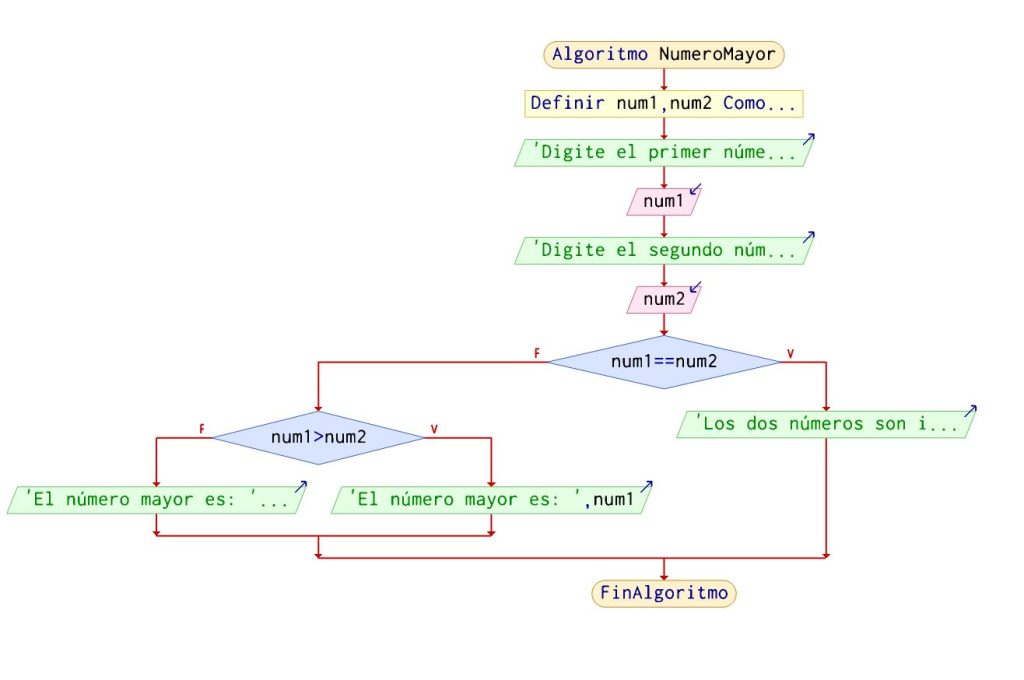
\includegraphics[width=0.95\linewidth]{00_IntroProgramacionYMoviles/DiagramaFlujo1.jpg} 
\end{center}
\end{columns}
\end{frame}

\begin{frame}
\frametitle{Codificacion de un algoritmo en varios lenguajes de programaci\'on (Python - Kotlin)} 
\begin{columns}
\column{0.45\linewidth}
\begin{block}{Codificacion del Algoritmo en Python}
\inputminted[linenos,fontsize=\tiny]{python}{00_IntroProgramacionYMoviles/Hello.py}
\end{block}
\column{0.45\linewidth}
\begin{block}{Codificacion del Algoritmo en Kotlin}
\inputminted[linenos,fontsize=\tiny]{python}{00_IntroProgramacionYMoviles/Hello.kt}
\end{block}
\end{columns}
\end{frame}



\begin{frame}
\frametitle{Sistema Operativo}  
\begin{columns}
%\column{0.32\linewidth}
\column{0.65\linewidth}
\begin{block}{}
Un Sistema Operativo (SO) es un programa (software) que al arrancar la computadora** se encarga de gestionar todos los recursos del sistema informático permitiendo así la comunicación entre el usuario y la computadora. 
\end{block}
\begin{center}
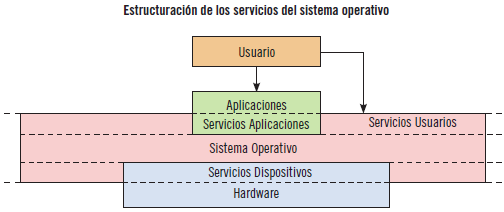
\includegraphics[width=0.95\linewidth]{00_IntroProgramacionYMoviles/SistemaOperativo1.png} 
\end{center}
\tiny{\url{https://reader.digitalbooks.pro/content/preview/books/38230/book/OEBPS/Text/c1.html}}

\column{0.32\linewidth}
\begin{center}
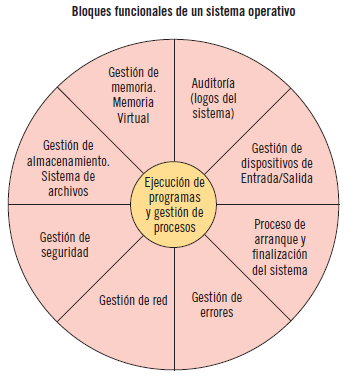
\includegraphics[width=0.95\linewidth]{00_IntroProgramacionYMoviles/SistemaOperativo2.png} 
\end{center}
\end{columns}

\end{frame}


\begin{frame}
\frametitle{Sistemas Operativos para PCs}  

\begin{columns}
\column{0.32\linewidth}
\begin{center}

\includegraphics[width=0.95\linewidth]{00_IntroProgramacionYMoviles/Windows11.png} 
\end{center}

\column{0.32\linewidth}
\begin{center}
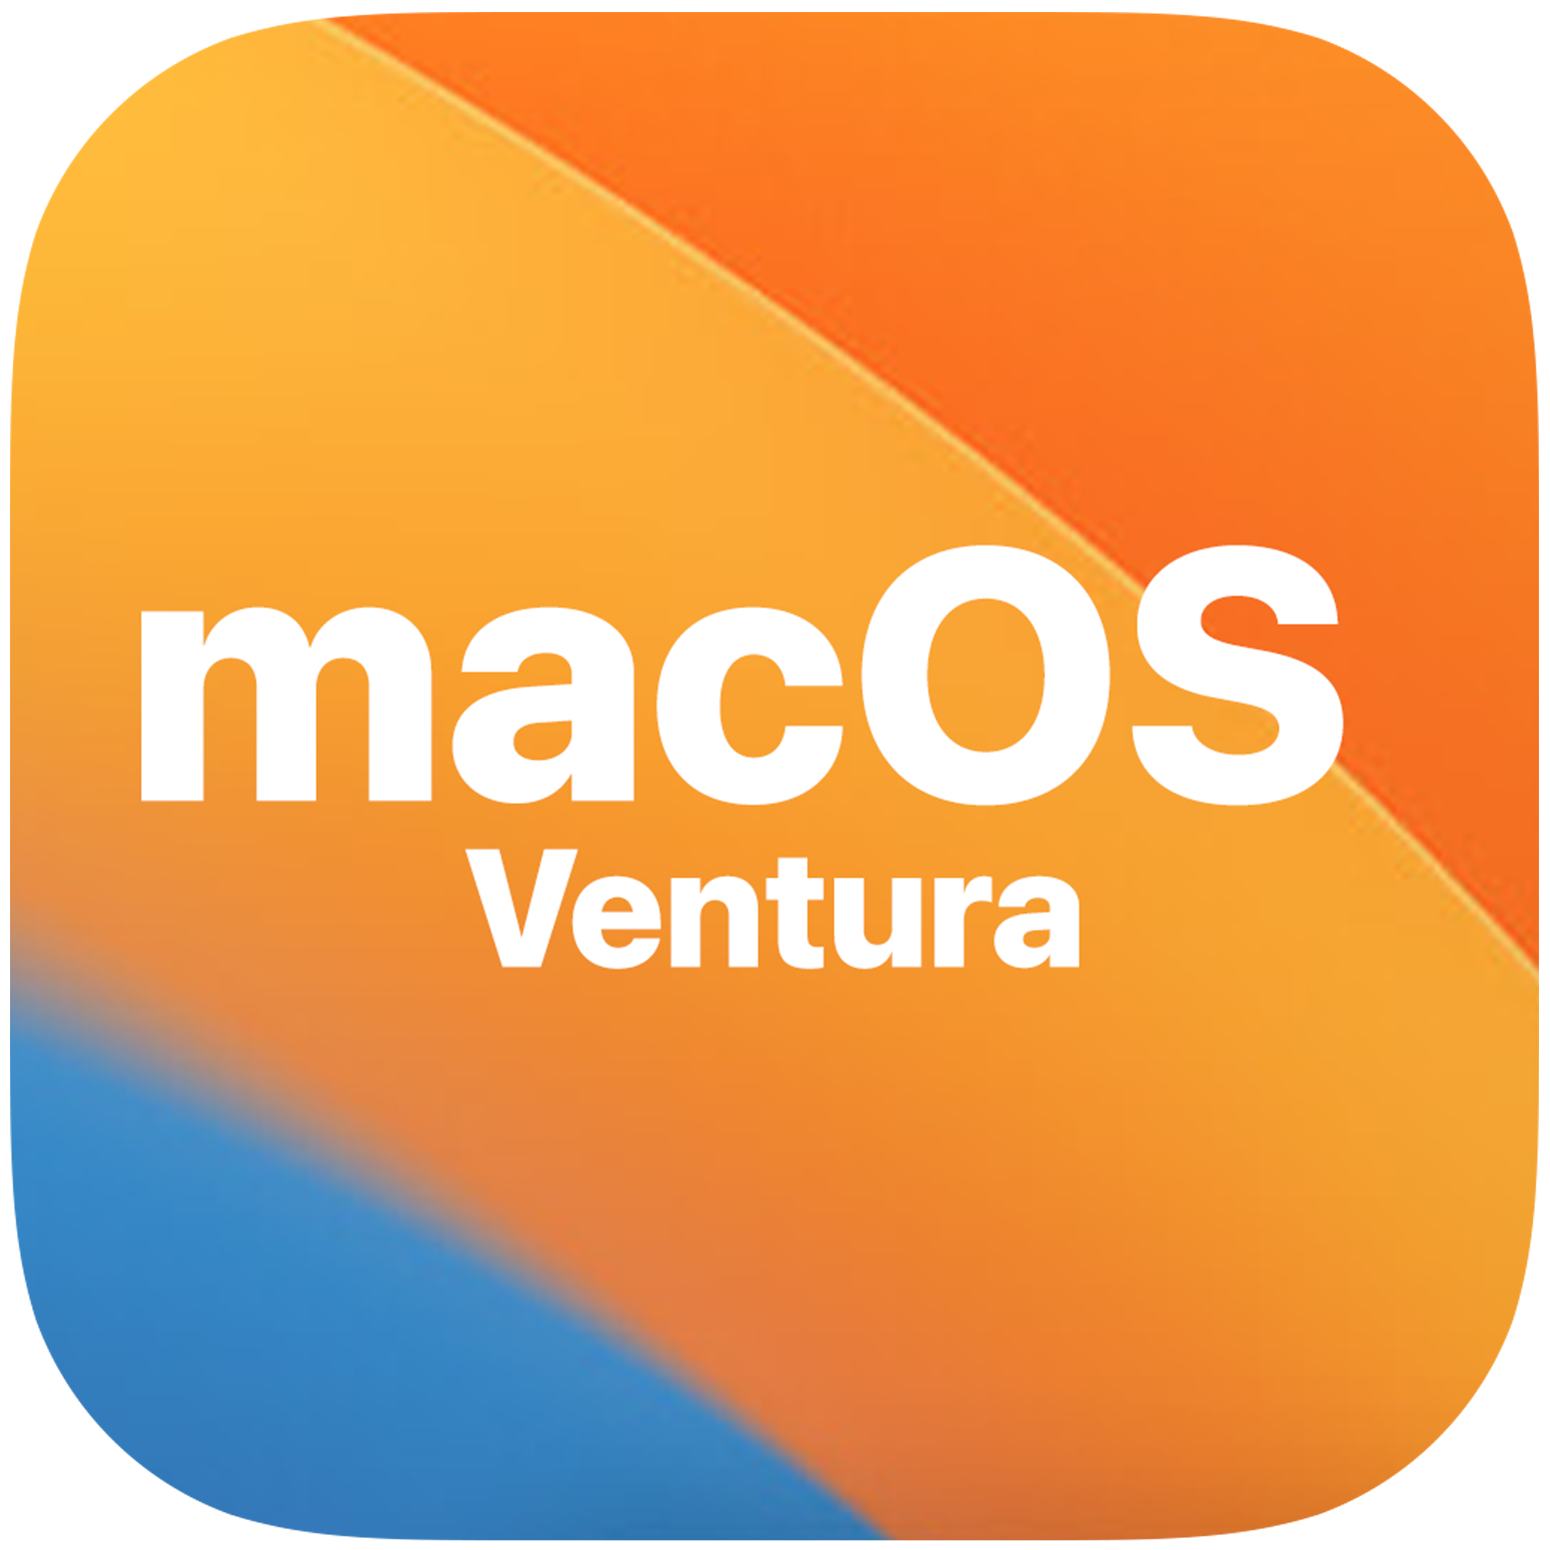
\includegraphics[width=0.95\linewidth]{00_IntroProgramacionYMoviles/MacOS.png} 
\end{center}

\column{0.32\linewidth}
\begin{center}

\includegraphics[width=0.95\linewidth]{00_IntroProgramacionYMoviles/Linux.png} 
\end{center}
\end{columns}

\end{frame}





\begin{frame}
\frametitle{Telefono Celular No-inteligente vs Telefono Celular Inteligente}  

\begin{columns}
\column{0.46\linewidth}
\begin{block}{Tel\'efono No-inteligente}
\begin{itemize}
\item Su funcionalidad principal era la comunicaci\'on (llamadas o mensajes) a trav\'es de la red celular (GSM)
\end{itemize}
\end{block}
\begin{block}{Tel\'efono inteligente}
\begin{itemize}
\item Interfaz de entrada: Pantalla Touch (a color, de alta definici\'on) 
\item Conexi\'on a Internet: WiFi, GSM (4G o 5G)
\item Comunicaci\'on con otros dispositivos: Bluetooth, NFC
\item C\'amaras (Frontal y Posterior)
\end{itemize}
\end{block}

\column{0.18\linewidth}
\begin{center}
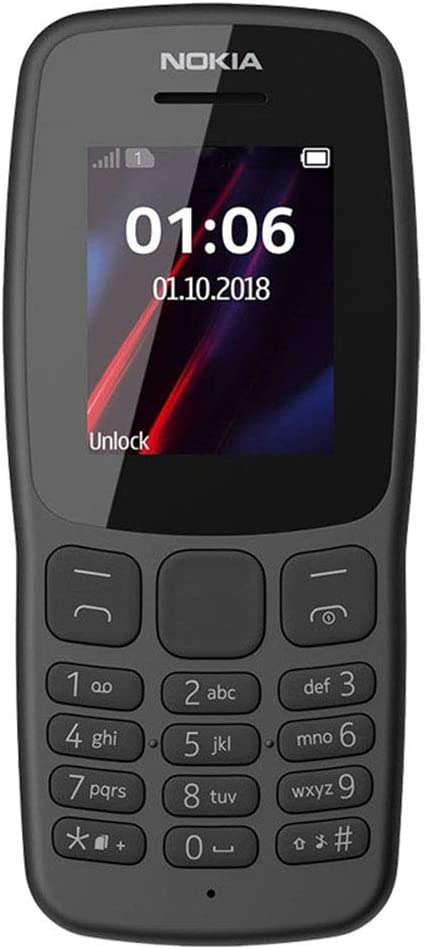
\includegraphics[width=0.95\linewidth]{00_IntroProgramacionYMoviles/FeaturePhone_Nokia.png} 
\end{center}
\column{0.28\linewidth}
\begin{center}
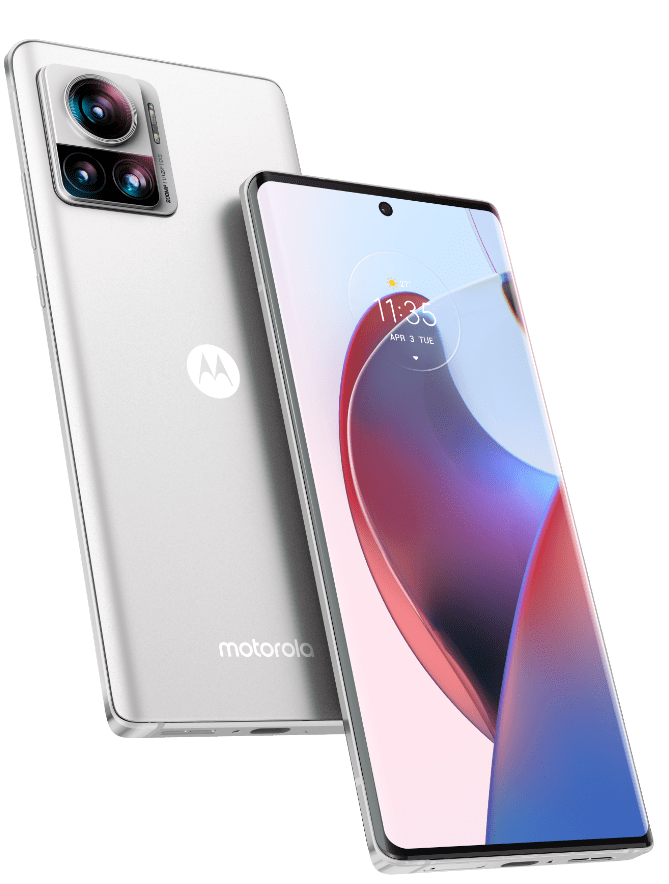
\includegraphics[width=0.95\linewidth]{00_IntroProgramacionYMoviles/Smartphone_Motorola.png} 
\end{center}
\end{columns}
\end{frame}

\begin{frame}
\frametitle{Sistemas Operativos para Telefonos Inteligentes} 
\begin{columns}
\column{0.32\linewidth}
\begin{center}

\includegraphics[width=0.95\linewidth]{00_IntroProgramacionYMoviles/Android.png} 
\end{center}

\column{0.32\linewidth}
\begin{center}
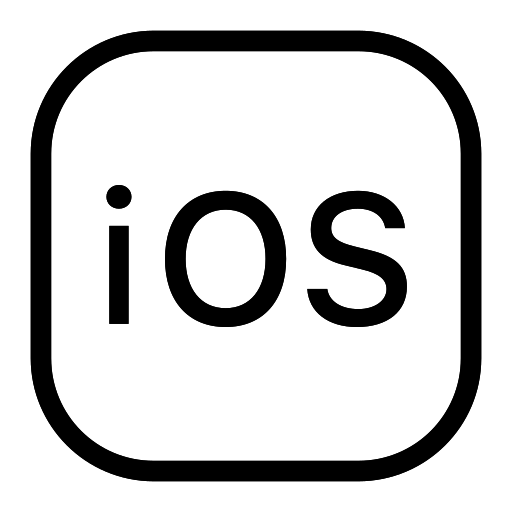
\includegraphics[width=0.95\linewidth]{00_IntroProgramacionYMoviles/iOs.png} 
\end{center}

\column{0.32\linewidth}
\begin{center}

\includegraphics[width=0.95\linewidth]{00_IntroProgramacionYMoviles/WindowsPhone.png} 
\end{center}
\end{columns}
 
\end{frame}


\begin{frame}
\frametitle{Android} 
\begin{columns}
\column{0.64\linewidth}
\begin{itemize}
\item Android es un sistema operativo móvil basado en Linux 
\item Principalmente orientado a dispositivos de pantalla t\'actil (Smartphone, tablets, smartwatches, etc)
\item Fue desarrollado por Android Inc (Adquirida por Google en 2005)
\item Vinculado con un grupo de empresas (HTC, Sony, Motorola, Samsung, LG, Lenovo, entre otras) para la creaci\'on de un SO com\'un para sus dispositivos
\item A la fecha (Q1 2023), los tel\'efonos con SO Android concentran mas del 70\% del mercado global. 
\end{itemize}
\column{0.32\linewidth}
\begin{center}
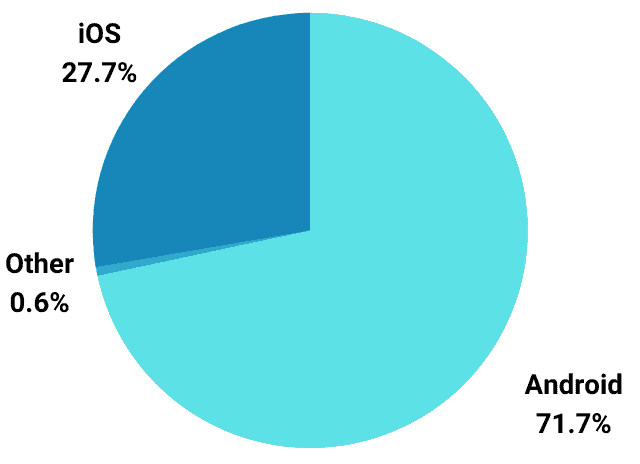
\includegraphics[width=0.95\linewidth]{00_IntroProgramacionYMoviles/AndroidVSIOs_WorldWide.png} 
\end{center}
\end{columns}
 
\end{frame}





\begin{frame}
\frametitle{Aplicaciones Móviles}  
\begin{columns}
\column{0.4\linewidth}
\begin{itemize}
\item Ejecutadas en el tel\'efono
\item La entrada de datos es mediante un teclado ``virtual''
\item El apuntador del raton es la pantalla 
\item Incluyen una interfaz de usuario gr\'afica (GUI) 
\item Es posible descargar miles de \'estas en nuestros dispositivos
\end{itemize}
\column{0.30\linewidth}
\begin{center}
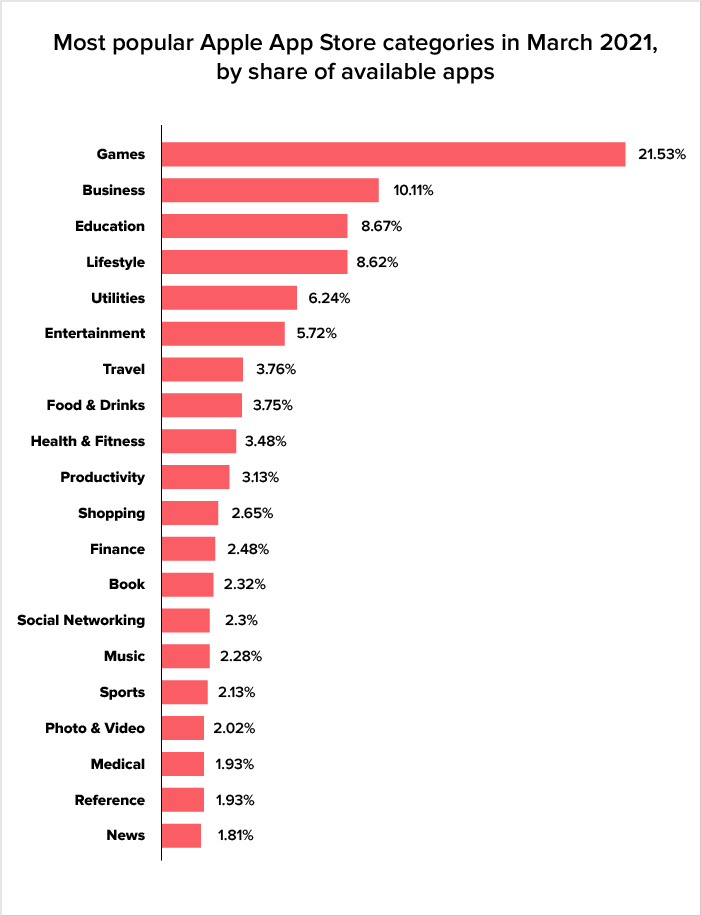
\includegraphics[width=0.95\linewidth]{00_IntroProgramacionYMoviles/TiposAplicaciones.png} 
\end{center}
\column{0.30\linewidth}
\begin{center}

\includegraphics[width=0.95\linewidth]{00_IntroProgramacionYMoviles/most-popular-apps.jpg} 
\tiny{\url{https://www.netsolutions.com/insights/top-10-most-popular-apps-2018/}}  
\end{center}
\end{columns}
\end{frame}


\begin{frame}
\frametitle{Android Studio}  

\begin{itemize}
\item Android Studio es un entorno oficial de desarrollo integrado (IDE) para el sistema operativo Android de Google
\item La primera versi\'on se libera en el año 2013, siendo el lenguaje de programacion Java
\item En 2019, se reemplaza el lenguaje oficial de desarrollo por Kotlin, aunque Java todav\'ia es soportado
\item Es gratis, se puede descargar e instalar en cualquier computadora sin importar el sistema operativo (Windows, Linux y MacOS)
\url{https://developer.android.com}
\end{itemize}
\end{frame}

%
\begin{frame}{Programación Móvil}
%\begin{block}{Programación Móvil} 
\begin{columns}
\begin{column}{0.98\textwidth}
    \begin{center}

\begin{itemize}
\item Es la actividad de desarrollar una aplicación específicamente para teléfonos inteligentes.
\item Estas aplicaciones se encuentran preinstaladas en el teléfono o pueden ser instaladas por el usuario mediante una tienda de aplicaciones (App Store o Google Play)
\item Las tareas que tradicionalmente hacíamos en la PC ahora están migrando hacia el teléfono inteligente
\item Principales sistemas operativos móviles: Android, iOS,
\item Enfocados principalmente en el desarrollo de aplicaciones NATIVAS.
\item Lenguajes de programación: Java, Kotlin.
\end{itemize}
     \end{center}

\end{column}
\end{columns}
%\end{block} 
\end{frame}


\begin{frame}
\frametitle{Codificacion de un algoritmo en varios lenguajes de programaci\'on (Python - Kotlin)} 
\begin{columns}
\column{0.45\linewidth}
\begin{block}{Codificacion del Algoritmo en Python}
\inputminted[linenos,fontsize=\tiny]{python}{00_IntroProgramacionYMoviles/Hello.py}
\end{block}
\column{0.45\linewidth}
\begin{block}{Codificacion del Algoritmo en Kotlin}
\inputminted[linenos,fontsize=\tiny]{python}{00_IntroProgramacionYMoviles/Hello.kt}
\end{block}
\end{columns}
\end{frame}



\begin{frame}
\frametitle{Sistema Operativo}  
\begin{columns}
%\column{0.32\linewidth}
\column{0.65\linewidth}
\begin{block}{}
Un Sistema Operativo (SO) es un programa (software) que al arrancar la computadora** se encarga de gestionar todos los recursos del sistema informático permitiendo así la comunicación entre el usuario y la computadora. 
\end{block}
\begin{center}
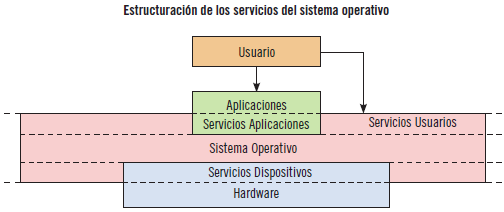
\includegraphics[width=0.95\linewidth]{00_IntroProgramacionYMoviles/SistemaOperativo1.png} 
\end{center}
\tiny{\url{https://reader.digitalbooks.pro/content/preview/books/38230/book/OEBPS/Text/c1.html}}

\column{0.32\linewidth}
\begin{center}
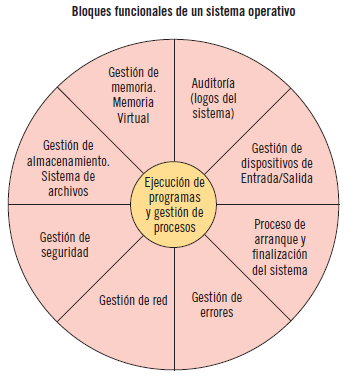
\includegraphics[width=0.95\linewidth]{00_IntroProgramacionYMoviles/SistemaOperativo2.png} 
\end{center}
\end{columns}

\end{frame}


\begin{frame}
\frametitle{Sistemas Operativos para PCs}  

\begin{columns}
\column{0.32\linewidth}
\begin{center}

\includegraphics[width=0.95\linewidth]{00_IntroProgramacionYMoviles/Windows11.png} 
\end{center}

\column{0.32\linewidth}
\begin{center}
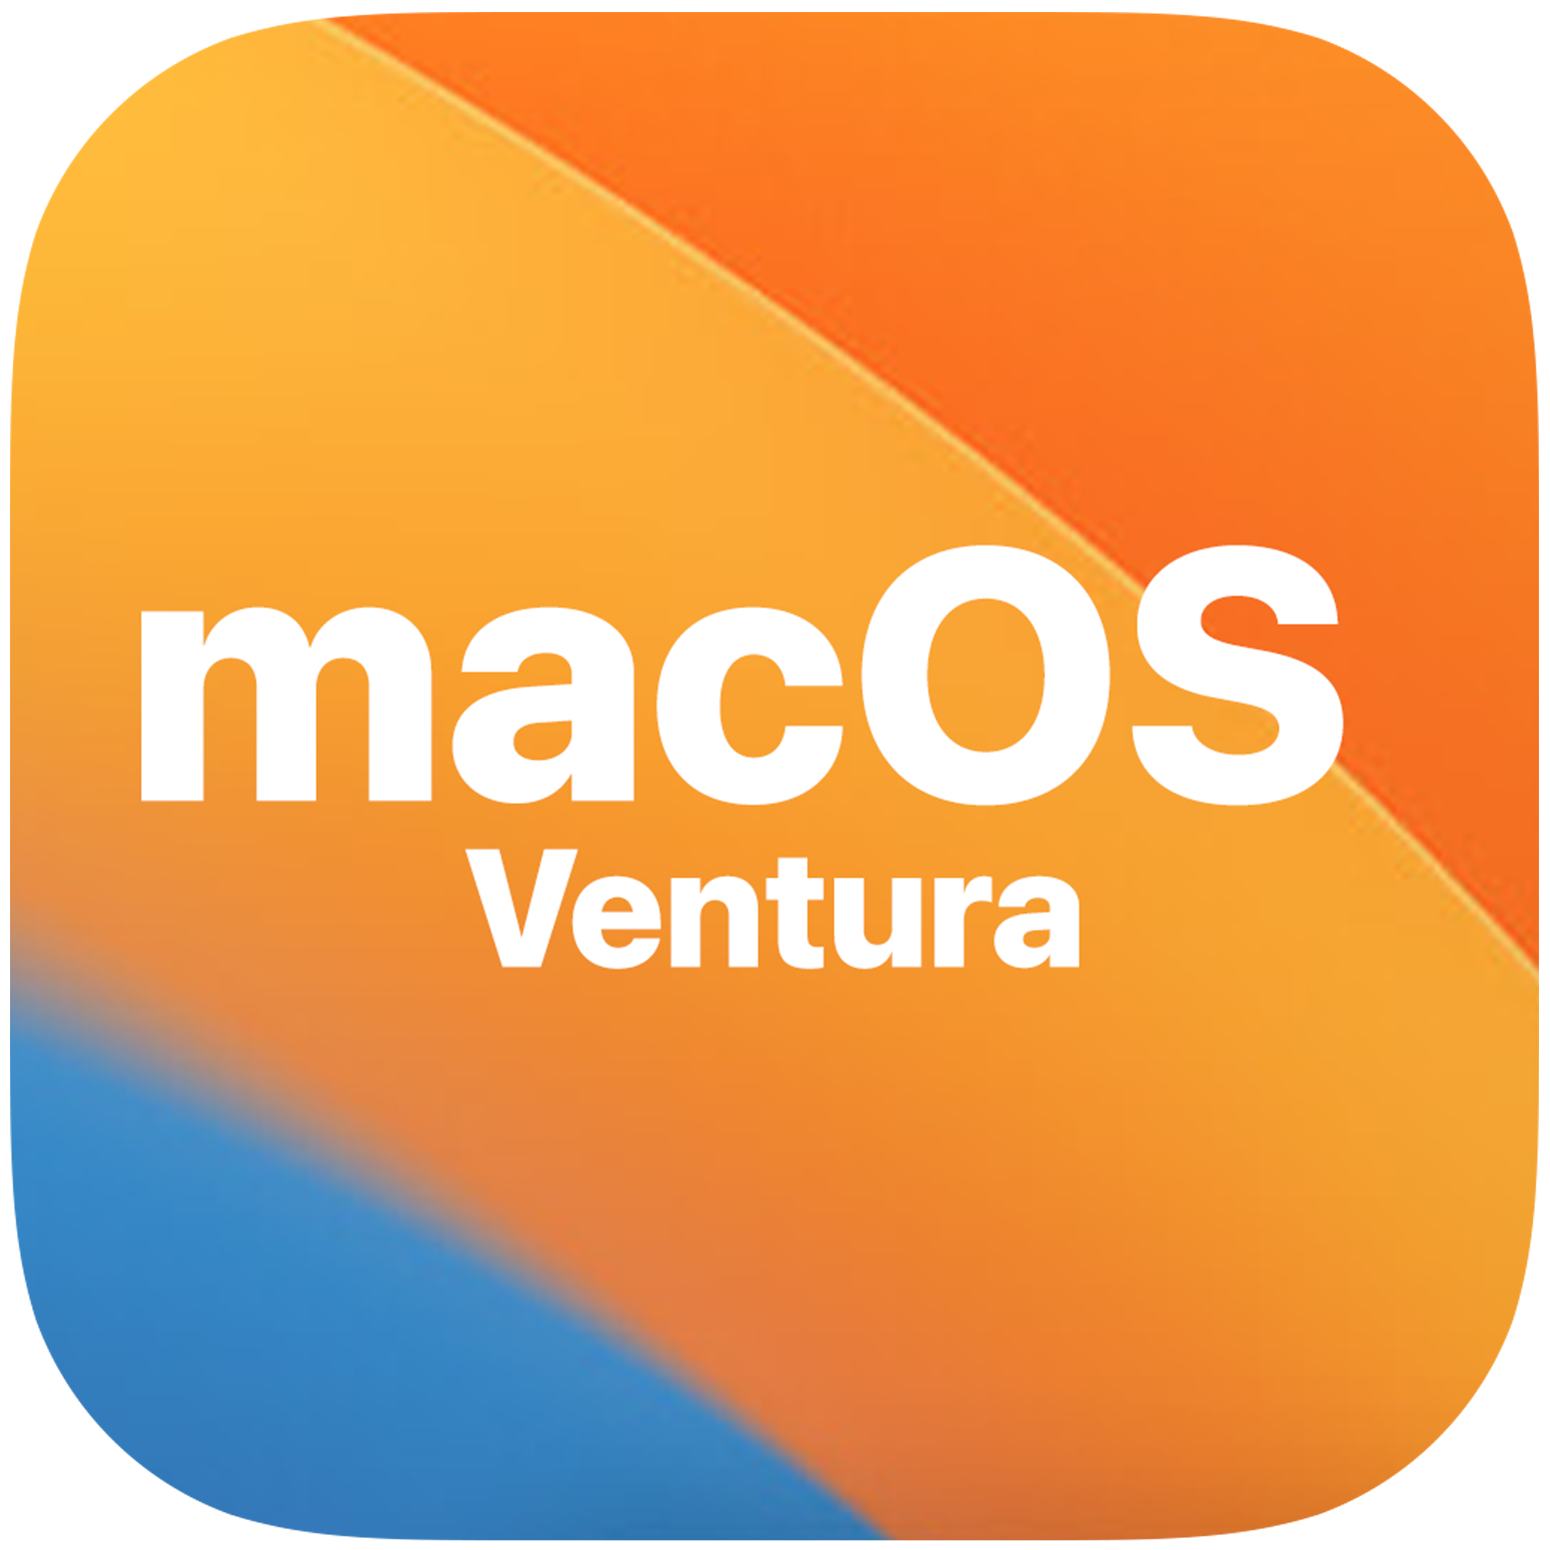
\includegraphics[width=0.95\linewidth]{00_IntroProgramacionYMoviles/MacOS.png} 
\end{center}

\column{0.32\linewidth}
\begin{center}

\includegraphics[width=0.95\linewidth]{00_IntroProgramacionYMoviles/Linux.png} 
\end{center}
\end{columns}

\end{frame}





\begin{frame}
\frametitle{Telefono Celular No-inteligente vs Telefono Celular Inteligente}  

\begin{columns}
\column{0.46\linewidth}
\begin{block}{Tel\'efono No-inteligente}
\begin{itemize}
\item Su funcionalidad principal era la comunicaci\'on (llamadas o mensajes) a trav\'es de la red celular (GSM)
\end{itemize}
\end{block}
\begin{block}{Tel\'efono inteligente}
\begin{itemize}
\item Interfaz de entrada: Pantalla Touch (a color, de alta definici\'on) 
\item Conexi\'on a Internet: WiFi, GSM (4G o 5G)
\item Comunicaci\'on con otros dispositivos: Bluetooth, NFC
\item C\'amaras (Frontal y Posterior)
\end{itemize}
\end{block}

\column{0.18\linewidth}
\begin{center}
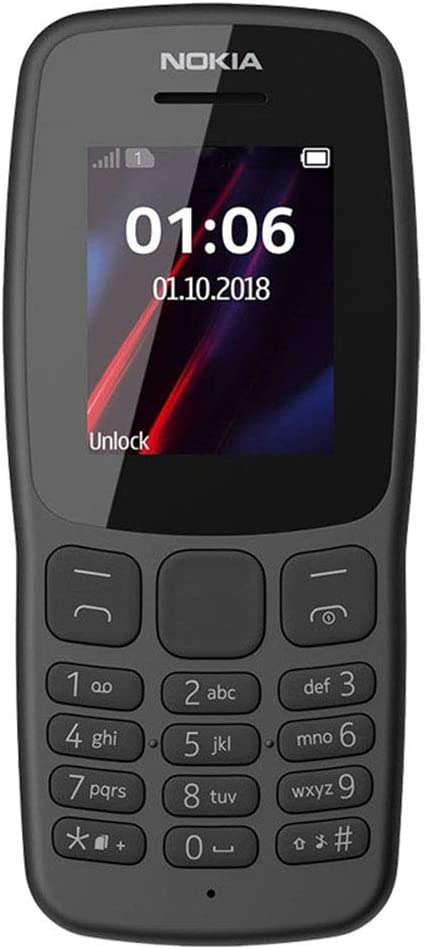
\includegraphics[width=0.95\linewidth]{00_IntroProgramacionYMoviles/FeaturePhone_Nokia.png} 
\end{center}
\column{0.28\linewidth}
\begin{center}
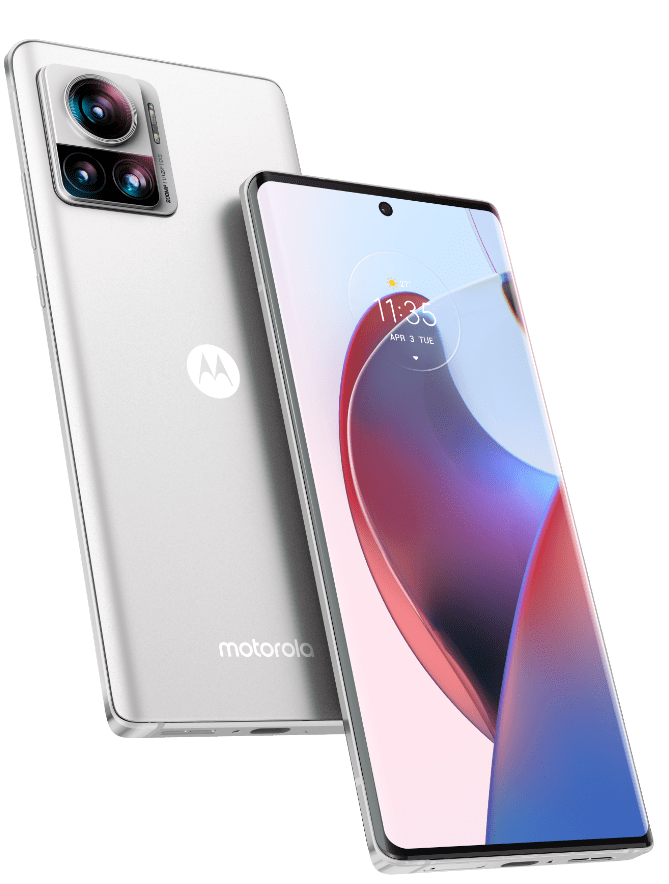
\includegraphics[width=0.95\linewidth]{00_IntroProgramacionYMoviles/Smartphone_Motorola.png} 
\end{center}
\end{columns}
\end{frame}

\begin{frame}
\frametitle{Sistemas Operativos para Telefonos Inteligentes} 
\begin{columns}
\column{0.32\linewidth}
\begin{center}

\includegraphics[width=0.95\linewidth]{00_IntroProgramacionYMoviles/Android.png} 
\end{center}

\column{0.32\linewidth}
\begin{center}
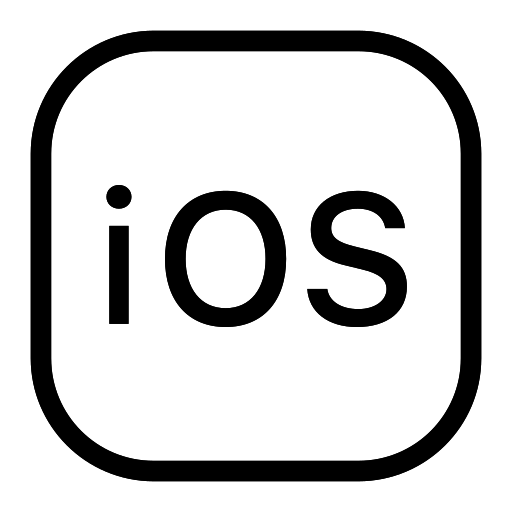
\includegraphics[width=0.95\linewidth]{00_IntroProgramacionYMoviles/iOs.png} 
\end{center}

\column{0.32\linewidth}
\begin{center}

\includegraphics[width=0.95\linewidth]{00_IntroProgramacionYMoviles/WindowsPhone.png} 
\end{center}
\end{columns}
 
\end{frame}


\begin{frame}
\frametitle{Android} 
\begin{columns}
\column{0.64\linewidth}
\begin{itemize}
\item Android es un sistema operativo móvil basado en Linux 
\item Principalmente orientado a dispositivos de pantalla t\'actil (Smartphone, tablets, smartwatches, etc)
\item Fue desarrollado por Android Inc (Adquirida por Google en 2005)
\item Vinculado con un grupo de empresas (HTC, Sony, Motorola, Samsung, LG, Lenovo, entre otras) para la creaci\'on de un SO com\'un para sus dispositivos
\item A la fecha (Q1 2023), los tel\'efonos con SO Android concentran mas del 70\% del mercado global. 
\end{itemize}
\column{0.32\linewidth}
\begin{center}
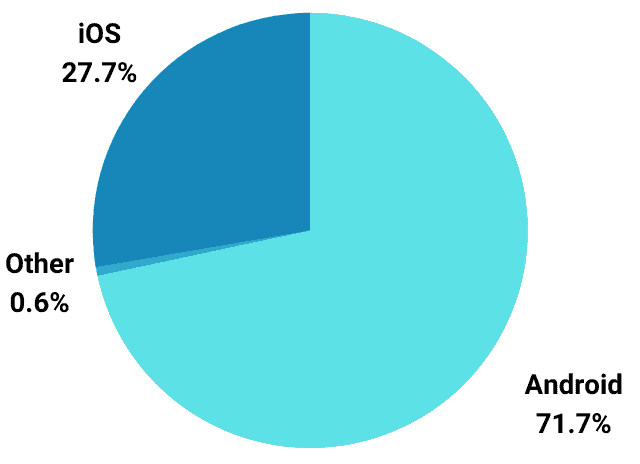
\includegraphics[width=0.95\linewidth]{00_IntroProgramacionYMoviles/AndroidVSIOs_WorldWide.png} 
\end{center}
\end{columns}
 
\end{frame}





\begin{frame}
\frametitle{Aplicaciones Móviles}  
\begin{columns}
\column{0.4\linewidth}
\begin{itemize}
\item Ejecutadas en el tel\'efono
\item La entrada de datos es mediante un teclado ``virtual''
\item El apuntador del raton es la pantalla 
\item Incluyen una interfaz de usuario gr\'afica (GUI) 
\item Es posible descargar miles de \'estas en nuestros dispositivos
\end{itemize}
\column{0.30\linewidth}
\begin{center}
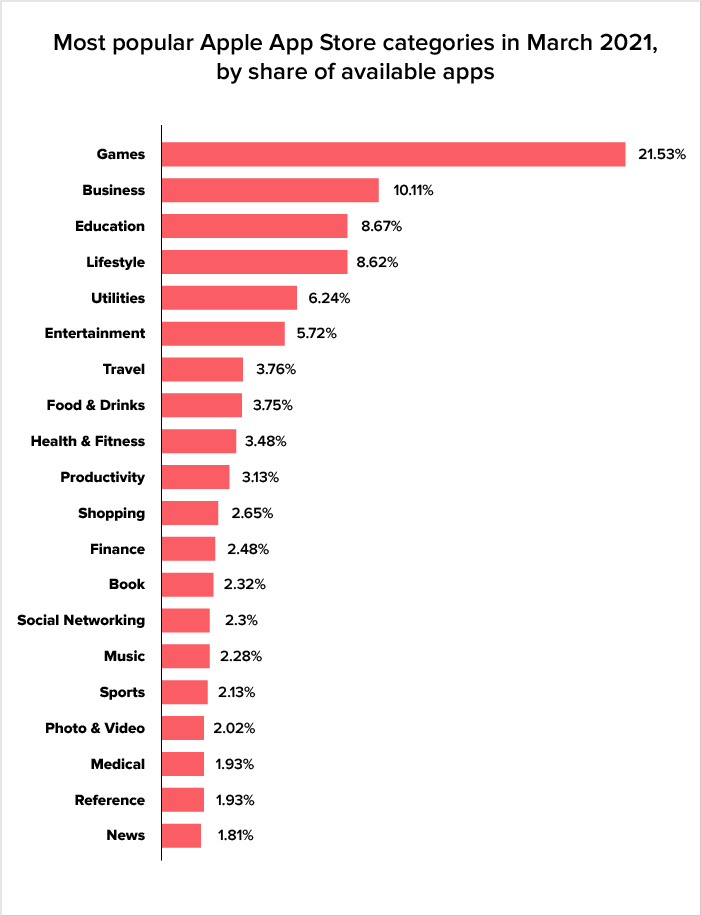
\includegraphics[width=0.95\linewidth]{00_IntroProgramacionYMoviles/TiposAplicaciones.png} 
\end{center}
\column{0.30\linewidth}
\begin{center}

\includegraphics[width=0.95\linewidth]{00_IntroProgramacionYMoviles/most-popular-apps.jpg} 
\tiny{\url{https://www.netsolutions.com/insights/top-10-most-popular-apps-2018/}}  
\end{center}
\end{columns}
\end{frame}


\begin{frame}
\frametitle{Android Studio}  

\begin{itemize}
\item Android Studio es un entorno oficial de desarrollo integrado (IDE) para el sistema operativo Android de Google
\item La primera versi\'on se libera en el año 2013, siendo el lenguaje de programacion Java
\item En 2019, se reemplaza el lenguaje oficial de desarrollo por Kotlin, aunque Java todav\'ia es soportado
\item Es gratis, se puede descargar e instalar en cualquier computadora sin importar el sistema operativo (Windows, Linux y MacOS)
\url{https://developer.android.com}
\end{itemize}
\end{frame}



\section[OpenGL]{OpenGL, GLSL y tecnologías asociadas}




% https://www.mathematik.uni-marburg.de/~thormae/lectures/graphics1/graphics_4_1_eng_web.html#1
\frame{
\frametitle{OpenGL}
\begin{itemize}
\item OpenGL significa Open Graphics Library, un estándar para la progamación gráfica.
\item Los comandos de gráficos son implementados por el controlador de la tarjeta gráfica y, por lo tanto, son independientes del hardware de la tarjeta gráfica, del sistema operativo y del administrador de ventanas empleado.
\item Los comandos de gráficos están cercanos hardware y son suficientes para lograr la funcionalidad principal
\item Varias bibliotecas y frameworks se basan en OpenGL y permiten la programación a un mayor nivel de abstracción.
\end{itemize}
}

\frame{
\frametitle{Versiones OpenGL para PC}
\begin{itemize}
\item Desde su introducción (1992) OpenGL se ha ampliado continuamente para admitir nuevas funciones de tarjetas gráficas.
\item OpenGL 1.0 (1992), OpenGL 1.1 (1997), OpenGL 1.2 (1998), OpenGL 1.3 (2001), OpenGL 1.4 (2002), OpenGL 1.5 (2003)
\item OpenGL 2.0 (2004), OpenGL 2.1 (2006)
\item OpenGL 3.0 (2008), OpenGL 3.1 (2009), OpenGL 3.2 (2009), OpenGL 3.3 (2010)
\item OpenGL 4.0 (2010), OpenGL 4.1 (2010), OpenGL 4.2 (2011), OpenGL 4.3 (2012), OpenGL 4.4 (2013), OpenGL 4.5 (2014), OpenGL 4.6 (2017)
%\item En esta ponencia, se combina la versi
\item A partir de la  versión 3.1, el Pipeline de funciones fijo ya no esta soportado, por l ocual es necesario implementar shaders, lo cual dificulta el aprendizaje.
\end{itemize}
}


\frame{
\frametitle{OpenGL ES y WebGL}
\begin{itemize}
\item OpenGL ES (Embedded System) es una versión de OpenGL con funcionalidad reducida para teléfonos móviles, televisores, tabletas, etc.
\item OpenGL ES 1.0 (2003): similar a OpenGL 1.3 (Pipeline Fijo)
\item OpenGL ES 1.1 (2004): similar a OpenGL 1.5 (compatible con versiones anteriores)
\item OpenGL ES 2.0 (2007): similar a OpenGL 2.0 (no compatible con versiones anteriores)
\item OpenGL ES 3.0 (2012): similar a OpenGL 3.3 
\item OpenGL ES 3.1 (2014): similar a OpenGL 4.3
\item OpenGL ES 3.2 (2015): similar a OpenGL 4.3
\item OpenGL ES 3.3 (2017): similar a OpenGL 4.6
\item WebGL esta basado en OpenGL ES 2.0 (y WebGL 2.0 en OpenGL ES 3.0) y permite gráficos 3D en páginas web (compatible con la mayoría de navegadores)
\end{itemize}
}

\begin{frame}{SoCs para Teléfonos Inteligentes}
\begin{columns}
\begin{column}{0.60\textwidth}  
\begin{itemize}
\item El término SoC significa system-on-a-chip.
\item Un SoC es un sistema completo contenido en un solo circuito integrado.
\item La combinación de todos sus componentes en una sola unidad de procesamiento permite un ahorro de energía significativo. 
\item Bloques comunes en un SoC:
\begin{itemize}
\item Central Processing Unit (CPU).
\item Graphics Processing Unit (GPU).
\item Image Processing Unit (ISP).
\item Digital Signal Processor (DSP).
\item Neural Processing Unit (NPU).
\item Video encoder/decoder.
\item Modems.
\end{itemize}
\end{itemize}
\end{column}
\begin{column}{0.40\textwidth}  
    \begin{center}
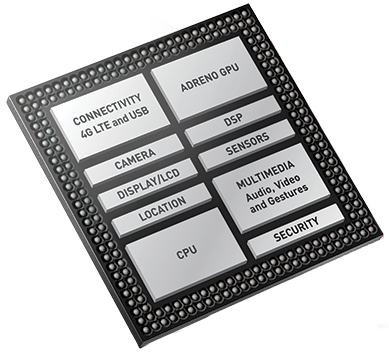
\includegraphics[width=0.65\textwidth]{FigsOpenGL/qualcomm_snapdragon410_block}\\
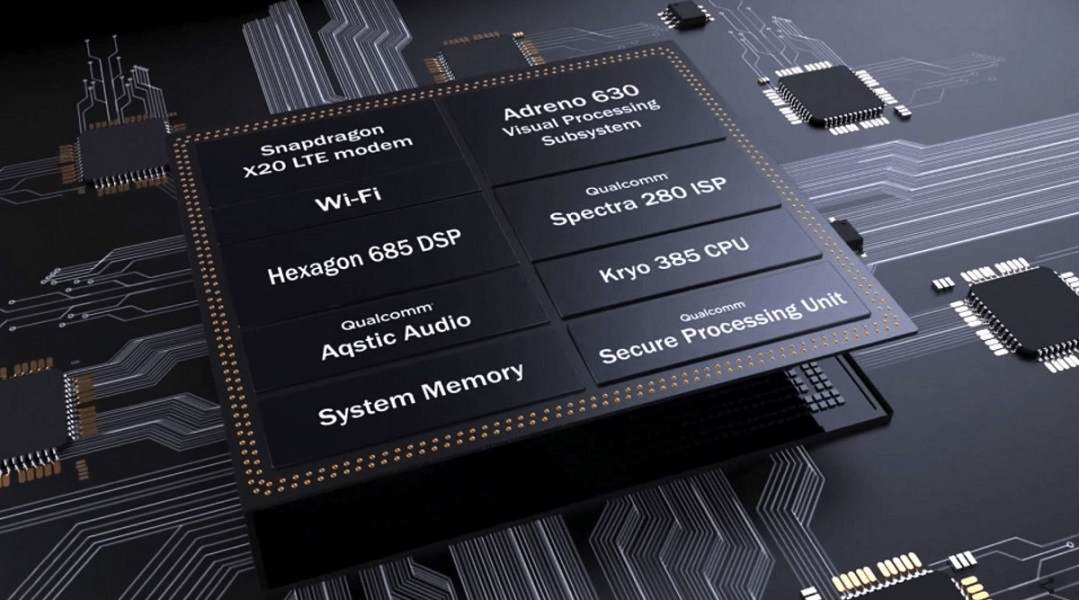
\includegraphics[width=0.85\textwidth]{FigsOpenGL/Snapdragon-855-1}
     \end{center}
\end{column}
\end{columns}
\end{frame}


\frame{
\frametitle{¿Qué es un GPU (Graphics Processing Unit)?}
\begin{columns}
\begin{column}{0.49\textwidth}
\begin{itemize}
\item Un GPU es un procesador formado por muchos núcleos más pequeños y especializados, especializada en operaciones de punto flotante en paralelo.
\item Al trabajar conjuntamente, los núcleos ofrecen un desempeño masivo cuando se puede dividir una tarea de procesamiento y es procesada por muchos núcleos.
\item Por ejemplo, el Samsung S10 utiliza un Qualcomm Snapdragon 855 SoC (tiene un CPU de 8 núcleos y un GPU dedidado para gráficos (Adreno 640).
\end{itemize}
\end{column}
\begin{column}{0.19\textwidth}
\begin{center}
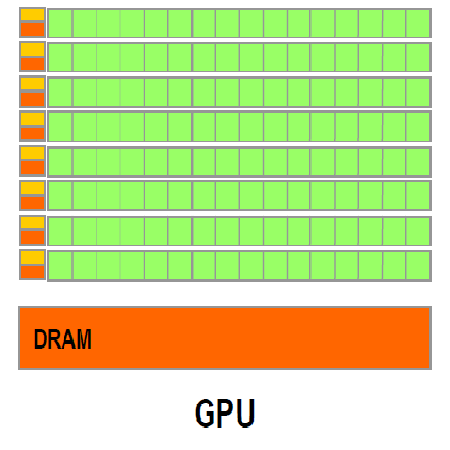
\includegraphics[width=0.9\textwidth]{FigsOpenGL/GPU}\\
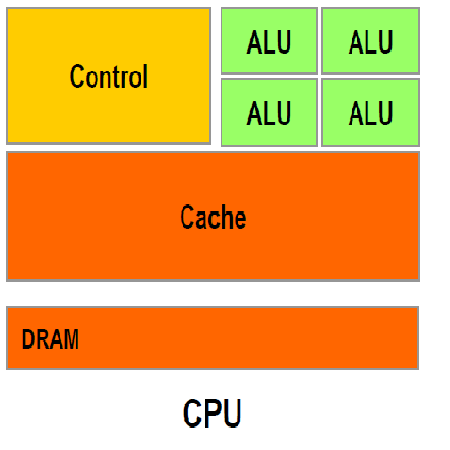
\includegraphics[width=0.9\textwidth]{FigsOpenGL/CPU}\\
\end{center}
\end{column}
\begin{column}{0.30\textwidth}  
    \begin{center}
     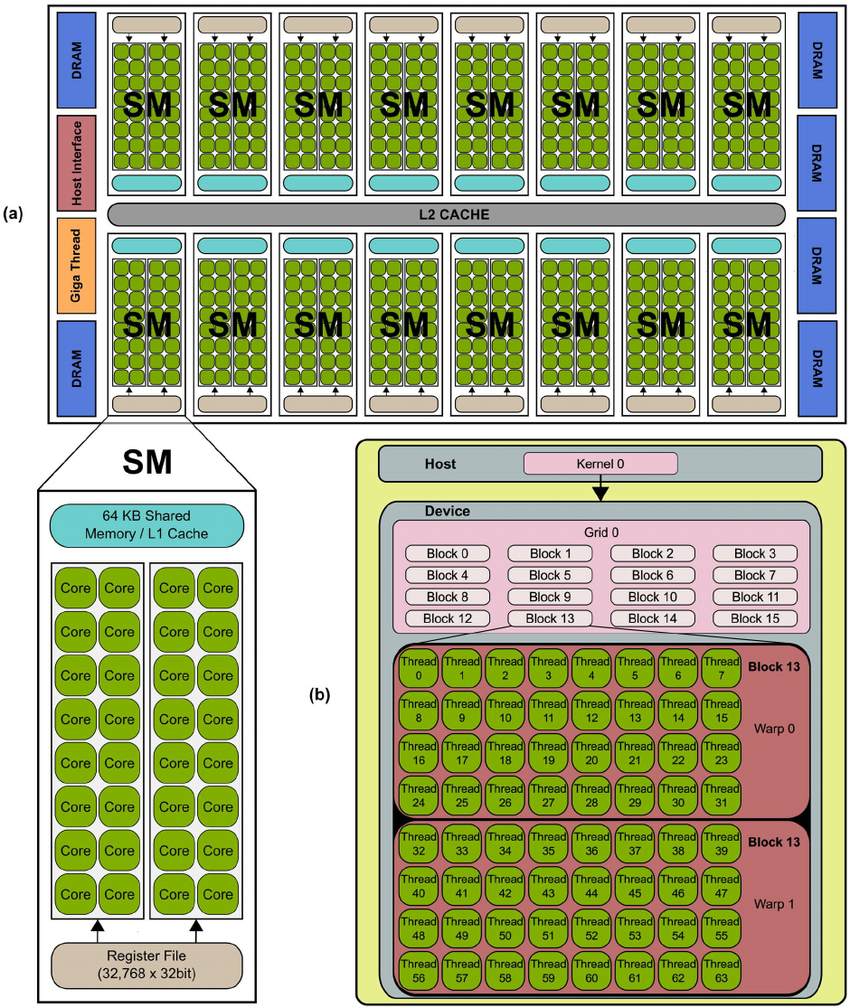
\includegraphics[width=\textwidth]{FigsOpenGL/Typical-NVIDIA-GPU-architecture}
     \end{center}
\end{column}
\end{columns}
}



%\begin{frame}{OpenGL}
%OpenGL signfiica Open Graphics Library, un estándar para la progamación de gráfica.
%El OpenGL Shading Language es un lengauje de alto nivel (cuya sintaxis es parecida a C) diseñado para procesamiento en paralelo en un GPU. 
%\end{frame}



\begin{frame}{OpenGL Pipeline}

\begin{columns}
\begin{column}{0.45\textwidth}
\begin{itemize}
\item Un Pipeline es una estructura de procesamiento paralelo
\item Un GPU tiene dos tipos de procesadores, incorporados en un Pipeline:
\begin{itemize}
\item El vertex processor
\item El fragment processor
\end{itemize}
\item Los programas son cargados en cada procesador.
\end{itemize}
\end{column}
\begin{column}{0.45\textwidth}
    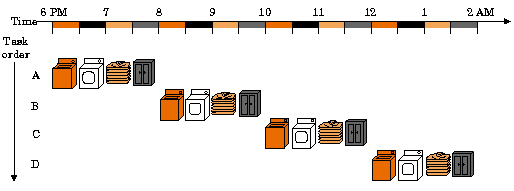
\includegraphics[width=\textwidth]{FigsOpenGL/Pipeline1.png}\\
    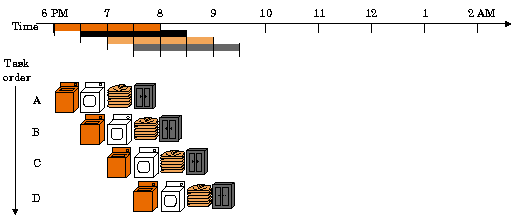
\includegraphics[width=\textwidth]{FigsOpenGL/Pipeline2.png}    
\end{column}
\end{columns}

\end{frame}


\begin{frame}{OpenGL Pipeline (2)}
    \begin{center}
    %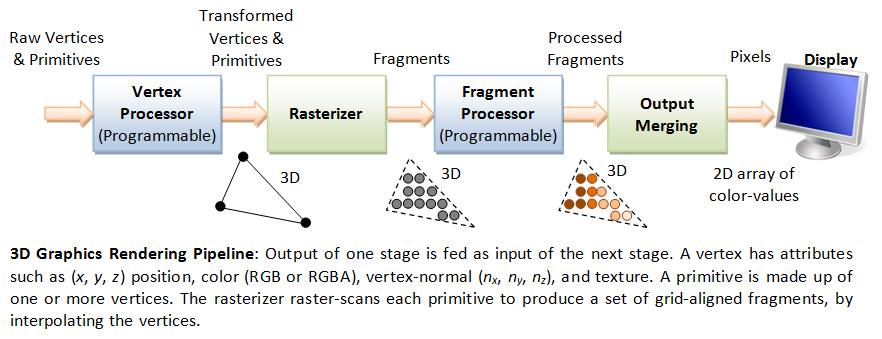
\includegraphics[width=\textwidth]{FigsOpenGL/Graphics3D_Pipe}
    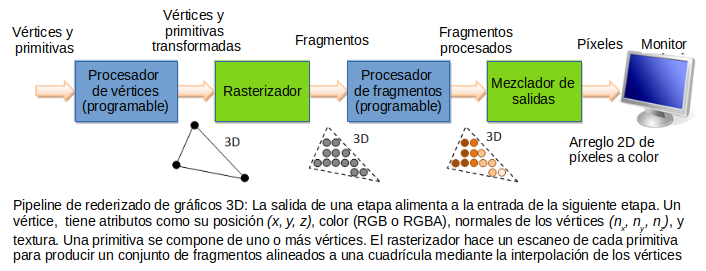
\includegraphics[width=\textwidth]{FigsOpenGL/OpenGL_Pipeline_Espaniol.png}
    \end{center}
\end{frame}


\begin{frame}{OpenGL Pipeline (3)}
    \begin{center}
    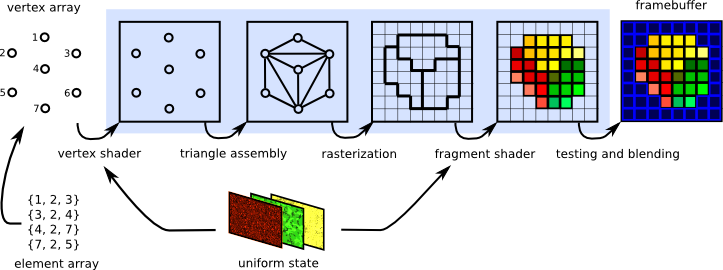
\includegraphics[width=\textwidth]{FigsOpenGL/evasgl-graphics-pipeline}
    \end{center}
\end{frame}

\begin{frame}{OpenGL Shading Language}
\begin{itemize}
\item Las aplicaciones móviles son ejecutadas principalmente en el CPU y la memoria principal
\item Para procesamiento de gráficos, los programas son ejecutados en el GPU el cual tiene su propia memoria local (memoria gráfica).
\item Los programas del GPU son escritos en un lenguaje llamado Shading Language (Lenguaje de sombreado). 
\item La mayoría de los GPUs adoptaron el lenguaje de OpenGL shading Language (OGSL)
\end{itemize}
\end{frame}

\begin{frame}{Transformaciones}
    \begin{center}
    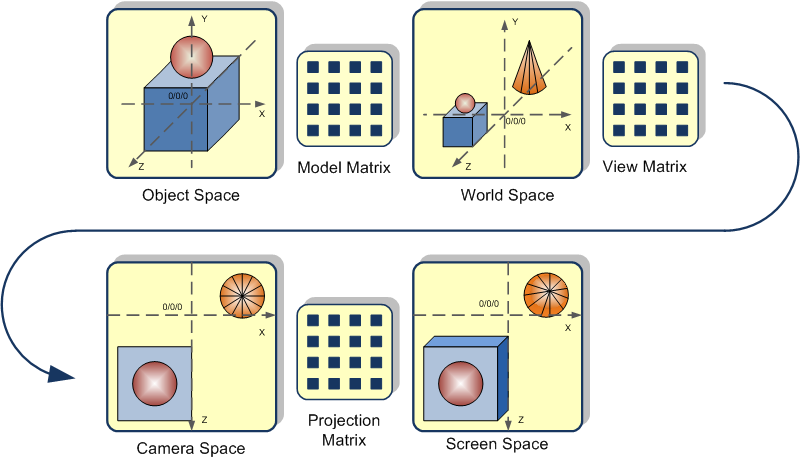
\includegraphics[width=0.75\textwidth]{FigsOpenGL/ModelViewProjection_MVP_Matrix}
    \end{center}
\end{frame}



\end{document}
%


\begin{frame}{Programación Móvil}
%\begin{block}{Programación Móvil} 
\begin{columns}
\begin{column}{0.98\textwidth}
    \begin{center}

\begin{itemize}
\item Es la actividad de desarrollar una aplicación específicamente para teléfonos inteligentes.
\item Estas aplicaciones se encuentran preinstaladas en el teléfono o pueden ser instaladas por el usuario mediante una tienda de aplicaciones (App Store o Google Play)
\item Las tareas que tradicionalmente hacíamos en la PC ahora están migrando hacia el teléfono inteligente
\item Principales sistemas operativos móviles: Android, iOS,
\item Enfocados principalmente en el desarrollo de aplicaciones NATIVAS.
\item Lenguajes de programación: Java, Kotlin.
\end{itemize}
     \end{center}

\end{column}
\end{columns}
%\end{block} 
\end{frame}


\begin{frame}
\frametitle{Sistema Operativo}  
\begin{columns}
%\column{0.32\linewidth}
\column{0.65\linewidth}
\begin{block}{}
Un Sistema Operativo (SO) es un programa (software) que al arrancar la computadora** se encarga de gestionar todos los recursos del sistema informático permitiendo así la comunicación entre el usuario y la computadora. 
\end{block}
\begin{center}
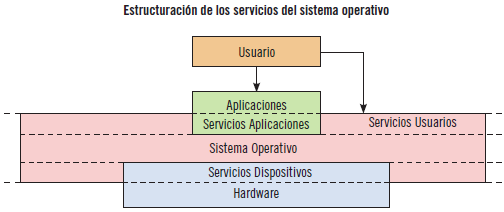
\includegraphics[width=0.95\linewidth]{00_IntroProgramacionYMoviles/SistemaOperativo1.png} 
\end{center}
\tiny{\url{https://reader.digitalbooks.pro/content/preview/books/38230/book/OEBPS/Text/c1.html}}

\column{0.32\linewidth}
\begin{center}
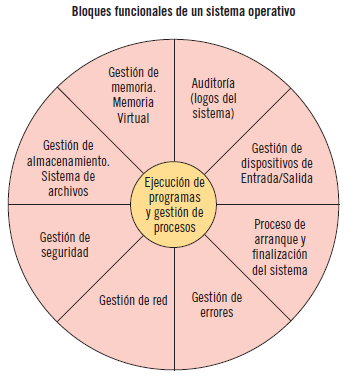
\includegraphics[width=0.95\linewidth]{00_IntroProgramacionYMoviles/SistemaOperativo2.png} 
\end{center}
\end{columns}

\end{frame}


\begin{frame}
\frametitle{Sistemas Operativos para PCs}  

\begin{columns}
\column{0.32\linewidth}
\begin{center}

\includegraphics[width=0.95\linewidth]{00_IntroProgramacionYMoviles/Windows11.png} 
\end{center}

\column{0.32\linewidth}
\begin{center}
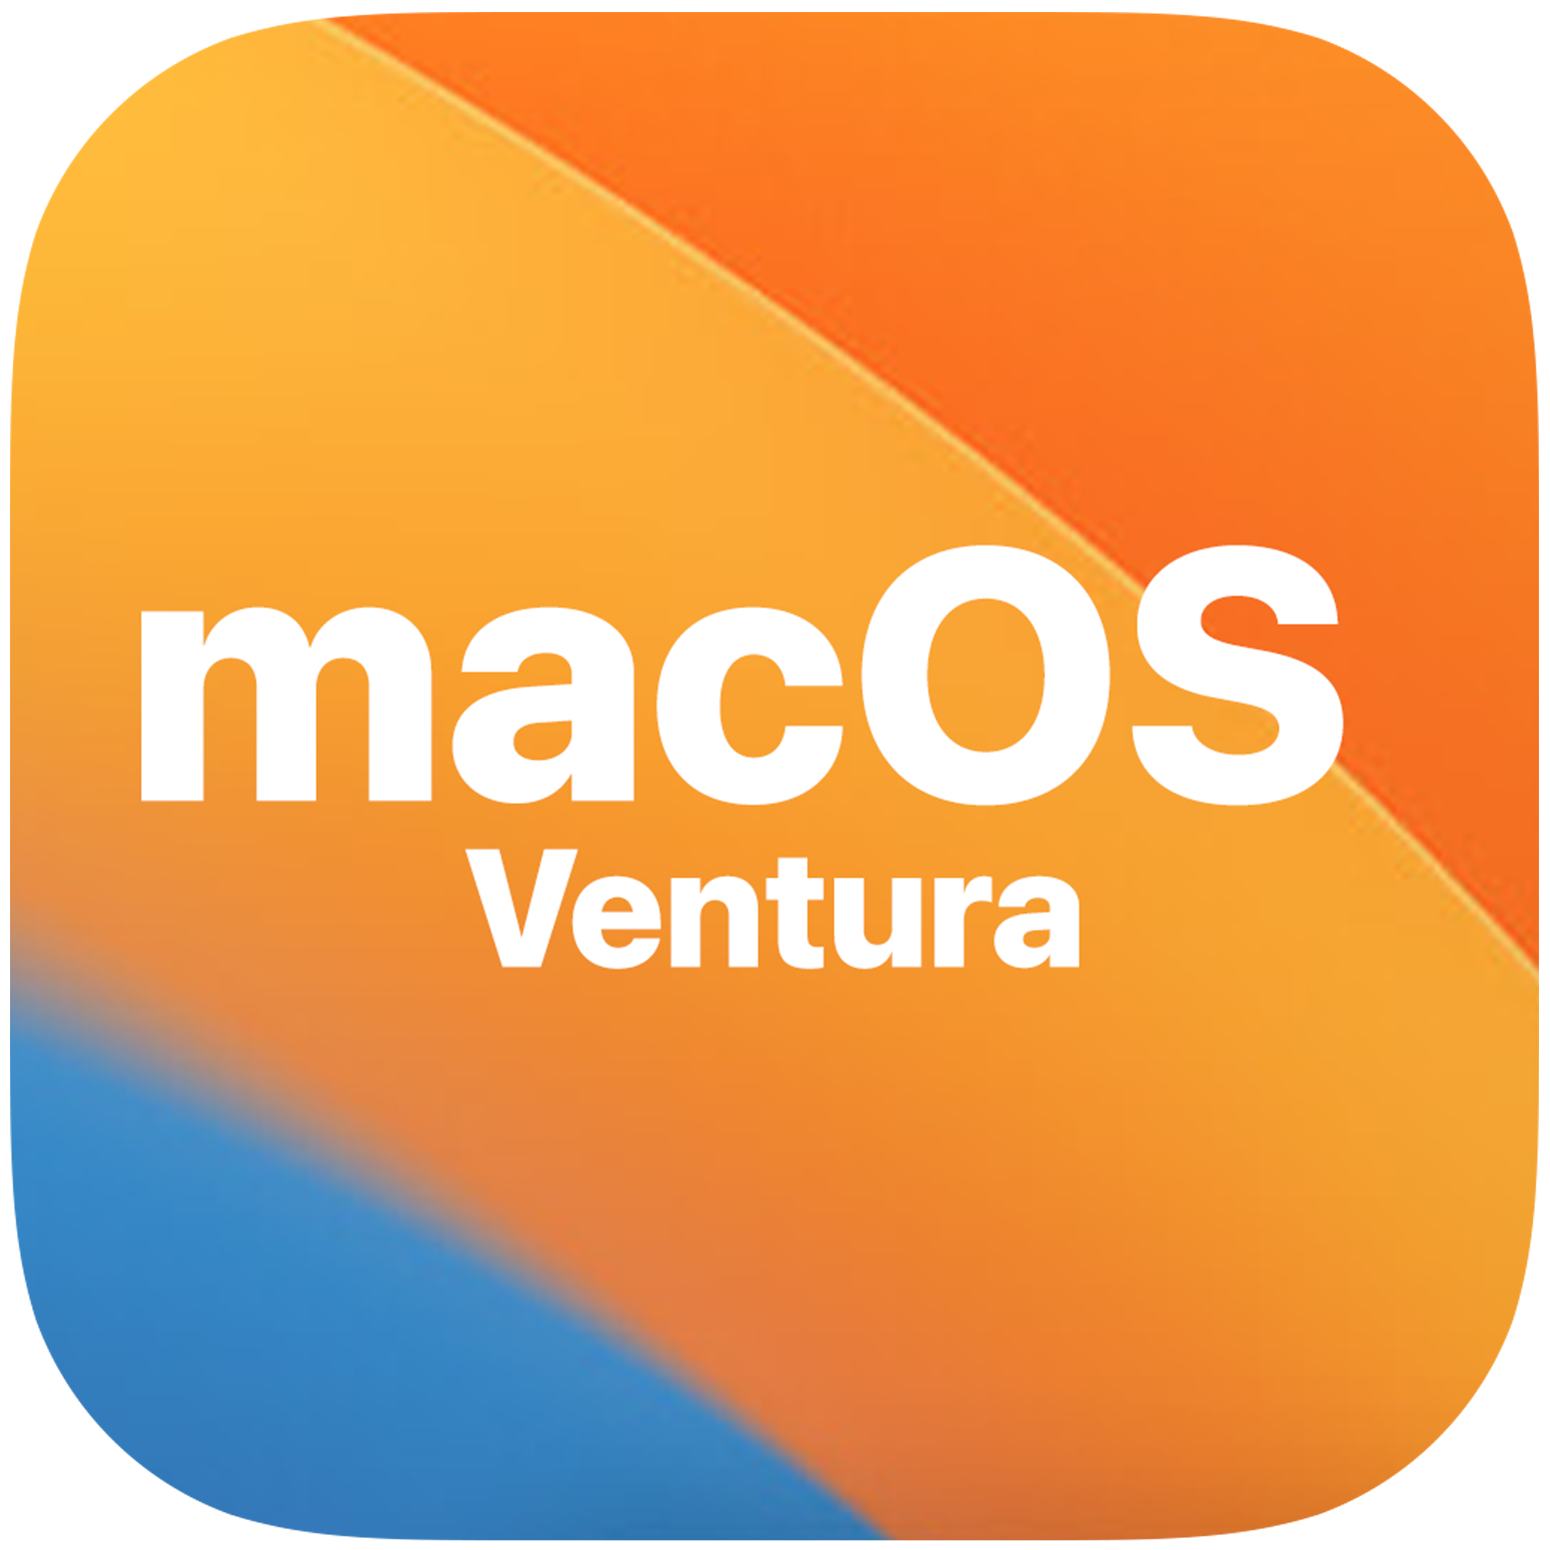
\includegraphics[width=0.95\linewidth]{00_IntroProgramacionYMoviles/MacOS.png} 
\end{center}

\column{0.32\linewidth}
\begin{center}

\includegraphics[width=0.95\linewidth]{00_IntroProgramacionYMoviles/Linux.png} 
\end{center}
\end{columns}

\end{frame}





\begin{frame}
\frametitle{Telefono Celular No-inteligente vs Telefono Celular Inteligente}  

\begin{columns}
\column{0.46\linewidth}
\begin{block}{Tel\'efono No-inteligente}
\begin{itemize}
\item Su funcionalidad principal era la comunicaci\'on (llamadas o mensajes) a trav\'es de la red celular (GSM)
\end{itemize}
\end{block}
\begin{block}{Tel\'efono inteligente}
\begin{itemize}
\item Interfaz de entrada: Pantalla Touch (a color, de alta definici\'on) 
\item Conexi\'on a Internet: WiFi, GSM (4G o 5G)
\item Comunicaci\'on con otros dispositivos: Bluetooth, NFC
\item C\'amaras (Frontal y Posterior)
\end{itemize}
\end{block}

\column{0.18\linewidth}
\begin{center}
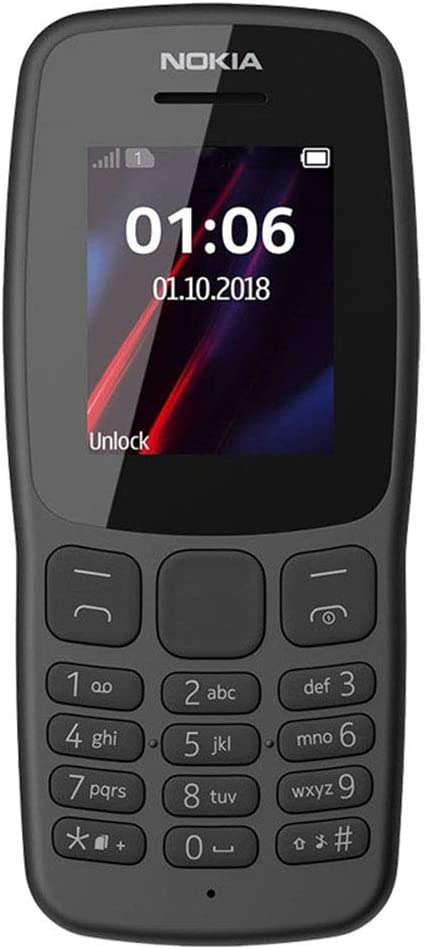
\includegraphics[width=0.95\linewidth]{00_IntroProgramacionYMoviles/FeaturePhone_Nokia.png} 
\end{center}
\column{0.28\linewidth}
\begin{center}
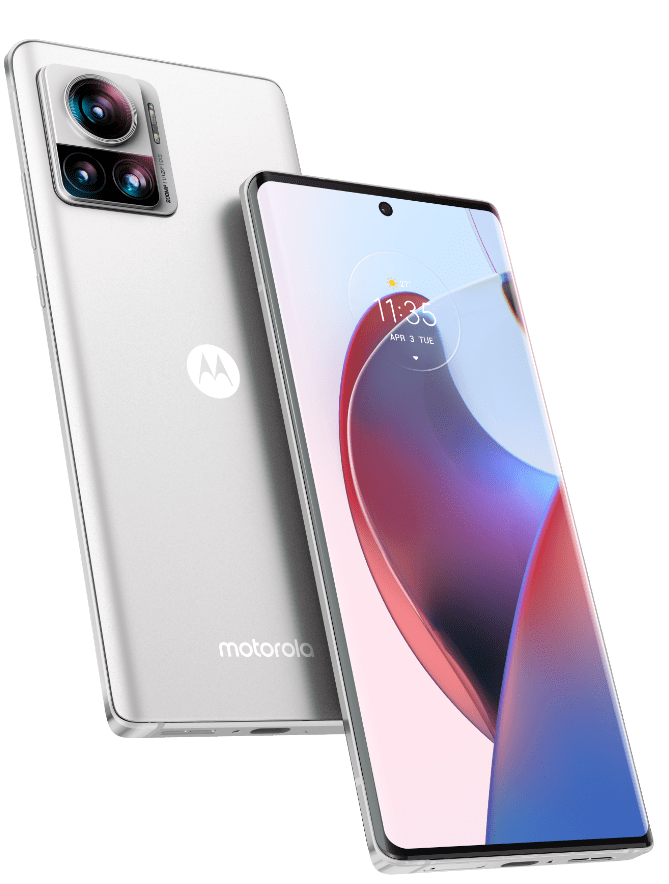
\includegraphics[width=0.95\linewidth]{00_IntroProgramacionYMoviles/Smartphone_Motorola.png} 
\end{center}
\end{columns}
\end{frame}

\begin{frame}
\frametitle{Sistemas Operativos para Telefonos Inteligentes} 
\begin{columns}
\column{0.32\linewidth}
\begin{center}

\includegraphics[width=0.95\linewidth]{00_IntroProgramacionYMoviles/Android.png} 
\end{center}

\column{0.32\linewidth}
\begin{center}
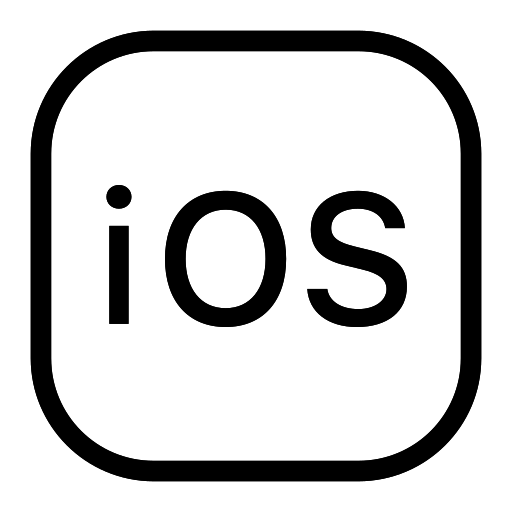
\includegraphics[width=0.95\linewidth]{00_IntroProgramacionYMoviles/iOs.png} 
\end{center}

\column{0.32\linewidth}
\begin{center}

\includegraphics[width=0.95\linewidth]{00_IntroProgramacionYMoviles/WindowsPhone.png} 
\end{center}
\end{columns}
 
\end{frame}


\begin{frame}
\frametitle{Android} 
\begin{columns}
\column{0.64\linewidth}
\begin{itemize}
\item Android es un sistema operativo móvil basado en Linux 
\item Principalmente orientado a dispositivos de pantalla t\'actil (Smartphone, tablets, smartwatches, etc)
\item Fue desarrollado por Android Inc (Adquirida por Google en 2005)
\item Vinculado con un grupo de empresas (HTC, Sony, Motorola, Samsung, LG, Lenovo, entre otras) para la creaci\'on de un SO com\'un para sus dispositivos
\item A la fecha (Q1 2023), los tel\'efonos con SO Android concentran mas del 70\% del mercado global. 
\end{itemize}
\column{0.32\linewidth}
\begin{center}
\includegraphics[width=0.95\linewidth]{00_IntroProgramacionYMoviles/AndroidVSIOs_WorldWide.png} 
\end{center}
\end{columns}
 
\end{frame}





\begin{frame}
\frametitle{Aplicaciones Móviles}  
\begin{columns}
\column{0.4\linewidth}
\begin{itemize}
\item Ejecutadas en el tel\'efono
\item La entrada de datos es mediante un teclado ``virtual''
\item El apuntador del raton es la pantalla 
\item Incluyen una interfaz de usuario gr\'afica (GUI) 
\item Es posible descargar miles de \'estas en nuestros dispositivos
\end{itemize}
\column{0.30\linewidth}
\begin{center}
\includegraphics[width=0.95\linewidth]{00_IntroProgramacionYMoviles/TiposAplicaciones.png} 
\end{center}
\column{0.30\linewidth}
\begin{center}
\includegraphics[width=0.95\linewidth]{00_IntroProgramacionYMoviles/most-popular-apps.jpg} 
\tiny{\url{https://www.netsolutions.com/insights/top-10-most-popular-apps-2018/}}  
\end{center}
\end{columns}
\end{frame}


\begin{frame}
\frametitle{Android Studio}  

\begin{itemize}
\item Android Studio es un entorno oficial de desarrollo integrado (IDE) para el sistema operativo Android de Google
\item La primera versi\'on se libera en el año 2013, siendo el lenguaje de programacion Java
\item En 2019, se reemplaza el lenguaje oficial de desarrollo por Kotlin, aunque Java todav\'ia es soportado
\item Es gratis, se puede descargar e instalar en cualquier computadora sin importar el sistema operativo (Windows, Linux y MacOS)
\url{https://developer.android.com}
\end{itemize}
\end{frame}

%
\section{Configurar smartphone en modo de Depuracion}

\begin{frame}
\frametitle{Configurar telefono inteligente en modo de desarrollador (0)}  
\begin{itemize}
\item Es necesario buscar en las opciones de configuraci\'on, en el apartado acerca del telefono ubicar el n\'umero de compilaci\'on 
\item Dar 5 taps (toques) sobre el n\'umero compilaci\'on. Debera aparecer un mensaje que diga que estas a X taps de ser un desarrollador 
\item Lo anterior habilita un nuevo men\'u en el apartado sistema dentro de opciones de configuraci\'on con t\'itulo ``opciones para desarrolladores'' 
\item Debe habilitarse tanto ``opciones para desarrolladores'' como la opci\'on ``depuraci\'on USB''
\end{itemize}

\end{frame}



\begin{frame}
\frametitle{Configurar telefono inteligente en modo de desarrollador (1)}  
\begin{columns}
\column{0.25\linewidth}
\begin{center}
\includegraphics[width=0.95\linewidth]{00_Configurar/ModoDesarrollador1.png}    
\end{center}
\column{0.25\linewidth}
\begin{center}
\includegraphics[width=0.95\linewidth]{00_Configurar/ModoDesarrollador2.png}    
\end{center}
\column{0.25\linewidth}
\begin{center}
\includegraphics[width=0.95\linewidth]{00_Configurar/ModoDesarrollador3.png}    
\end{center}
\column{0.25\linewidth}
\begin{center}
\includegraphics[width=0.95\linewidth]{00_Configurar/ModoDesarrollador4.png}    
\end{center}


\end{columns}

\end{frame}


\begin{frame}
\frametitle{Configurar telefono inteligente en modo de desarrollador (2)}  
\begin{columns}
\column{0.25\linewidth}
\begin{center}
\includegraphics[width=0.95\linewidth]{00_Configurar/ModoDesarrollador5.png}    
\end{center}
\column{0.25\linewidth}
\begin{center}
\includegraphics[width=0.95\linewidth]{00_Configurar/ModoDesarrollador6.png}    
\end{center}
\column{0.25\linewidth}
\begin{center}
\includegraphics[width=0.95\linewidth]{00_Configurar/ModoDesarrollador7.png}    
\end{center}
\column{0.25\linewidth}
\begin{center}
\includegraphics[width=0.95\linewidth]{00_Configurar/ModoDesarrollador8.png}    
\end{center}
\end{columns}
\end{frame}

\begin{frame}
\frametitle{Configurar telefono inteligente en modo de desarrollador (3)}  
\begin{columns}
\column{0.75\linewidth}

\begin{itemize}
\item Al habilitar la depuracion, aparece un mensaje de advertencia
\item Una vez que hayas terminado tus pruebas, se recomienda deshabilitar este modo de depuraci\'on
\item Para poder instalar una aplicaci\'on desarrollada con Android Studio, se debe conectar el tel\'efono inteligente a la computadora usando un cable USB
\end{itemize}

\column{0.25\linewidth}
\begin{center}
\includegraphics[width=0.95\linewidth]{00_Configurar/PermitirHabiliarOpcionesDesarrollo.jpg}    
\end{center}
\end{columns}
\end{frame}



\begin{frame}
\frametitle{Conectar smartphone a la computadora (Cable USB)}  
\begin{columns}
\column{0.25\linewidth}
\begin{itemize}
\item Al conectar el dispositivo por primera vez, aparece un mensaje de confirmaci\'on en el dispositivo
\item Configurar el telefono para que se conecte en modo de transferencia de archivos (por defecto, esta cargando)
\end{itemize}

\column{0.25\linewidth}
\begin{center}
\includegraphics[width=0.95\linewidth]{00_Configurar/HabilitarDepuracionUSB2.jpg}    
\end{center}

\column{0.25\linewidth}
\begin{center}
\includegraphics[width=0.95\linewidth]{00_Configurar/ModoConexion1.png}    
\end{center}

\column{0.25\linewidth}
\begin{center}
\includegraphics[width=0.95\linewidth]{00_Configurar/ModoConexion2.png}    
\end{center}
\end{columns}
\end{frame}



\begin{frame}
\frametitle{Ejecutar proyecto en telefono inteligente} 
\begin{columns}

\column{0.75\linewidth}
\begin{itemize}
\item Una vez conectado el telefono, debe aparecer el modelo en la parte superior (lado derecho) de tu proyecto de Android Studio
\item Para instalar la aplicacion en el telefono, deber dar click en una flecha verde justo a un lado de nombre del telefono (sean pacientes, puede tardar un poco la primera vez)
\end{itemize}
\begin{center}
\includegraphics[width=0.65\linewidth]{00_Configurar/AndroidStudio_SmartphoneReconocido.png}    
\end{center}
\column{0.25\linewidth}
\begin{center}
\includegraphics[width=0.95\linewidth]{00_Configurar/Etapa1_fase1.png}    
\end{center}
\end{columns} 
\end{frame}


%
\section{Crear primer proyecto en Android Studio}

\begin{frame}
\frametitle{Crear un primer proyecto (1)}  
\begin{columns}
\column{0.50\linewidth}
\begin{itemize}
\item Buscar el icono de la aplicacion y dar doble click
\item En caso de que requiera algunas actualizaciones, ser paciente, puede tardar.
\item Aparecera una ventana como la mostrada, seleccionar la opci\'on ``New project''
\end{itemize}
\column{0.50\linewidth}
\begin{center}
\includegraphics[width=0.95\linewidth]{00_PasosParaConfigurarSmartphoneModoDesarrollador/AndroidStudio01.png}    
\end{center}
\end{columns}
\end{frame}

\begin{frame}
\frametitle{Crear un primer proyecto (2)}  
\begin{columns}
\column{0.50\linewidth}
\begin{itemize}
\item Existen varios tipos de dispositivos para los que pueden crearse proyectos. Por defecto nos ubica en el primer grupo (Phone and Tablet)
\item Seleccionar tipo de proyecto  ``Empty Views Activity'' y dack click en Next
\end{itemize}
\column{0.50\linewidth}
\begin{center}
\includegraphics[width=0.95\linewidth]{00_PasosParaConfigurarSmartphoneModoDesarrollador/AndroidStudio02.png}    
\end{center}
\end{columns}
\end{frame}

\begin{frame}
\frametitle{Crear un primer proyecto (3)}  
\begin{columns}
\column{0.50\linewidth}
\begin{itemize}
\item Dejar los valores por defecto, solo se suguiere cambiar el nombre del proyecto
\item \textbf{Debe estar seleccionado como lenguaje Kotlin}. De estar seleccionado uno diferente, cambiar
\item Presionar el boton Finish
\end{itemize}
\column{0.50\linewidth}
\begin{center}
\includegraphics[width=0.95\linewidth]{00_PasosParaConfigurarSmartphoneModoDesarrollador/AndroidStudio03.png}    
\end{center}
\end{columns}
\end{frame}

\begin{frame}
\frametitle{Crear un primer proyecto (4)}  
\begin{columns}
\column{0.50\linewidth}
\begin{itemize}
\item La primera vez que se crea un proyecto, puede requerir la descarga de archivos necesarios. Le recomiendo ser paciente
\item Ya una vez que el proyecto fue creado, aparece la ventana mostrada
\end{itemize}
\column{0.50\linewidth}
\begin{center}
\includegraphics[width=0.95\linewidth]{00_PasosParaConfigurarSmartphoneModoDesarrollador/AndroidStudio04.png}    
\end{center}
\end{columns}
\end{frame}


%\section{Modificacion de la Interfaz de usuario}


\begin{frame}
\frametitle{Carpetas del proyecto}
\begin{columns}
\column{0.75\linewidth}
Carpetas y archivos importantes
\begin{itemize}
\item \textit{Manifest} - Por el momento es de interes
\item \textit{Java} - C\'odigo fuente - Dentro hay un archivo \textit{MainActivity.kt}
\item \textit{Res} - Recursos (im\'agenes) y definici\'on de interfaces. Dentro hay una carpeta llamada \textit{layout}, con un archivo \textit{activity\_main.xml}
\end{itemize}
\column{0.25\linewidth}
\begin{center}
\includegraphics[width=0.95\linewidth]{00_Modificacion/PanelCarpetas.png}    
\end{center}
\end{columns}   
\end{frame}


%\section{Agregar Codigo a la Interfaz}
\begin{frame}[fragile]
\frametitle{Agregar codigo a la interfaz}  


\begin{columns}

\column{0.50\linewidth}
\textit{Apariencia}
\begin{block}{Archivo \textbf{activity\_main.xml}}
\begin{minted}[linenos,fontsize=\tiny]{xml}
<?xml version="1.0" encoding="utf-8"?>
<androidx.constraintlayout.widget.ConstraintLayout 
    xmlns:android="http://schemas.android.com/apk/res/android"
    xmlns:app="http://schemas.android.com/apk/res-auto"
    xmlns:tools="http://schemas.android.com/tools"
    android:layout_width="match_parent"
    android:layout_height="match_parent"
    tools:context=".MainActivity">
    <TextView
        android:layout_width="wrap_content"
        android:layout_height="wrap_content"
        android:text="Hello World!"
        app:layout_constraintBottom_toBottomOf="parent"
        app:layout_constraintEnd_toEndOf="parent"
        app:layout_constraintStart_toStartOf="parent"
        app:layout_constraintTop_toTopOf="parent" />
</androidx.constraintlayout.widget.ConstraintLayout>
\end{minted}

\end{block}

\column{0.48\linewidth}
\textit{Comportamento}
\begin{block}{Archivo \textbf{MainActivity.kt}}
\begin{minted}[linenos,fontsize=\tiny]{kotlin}
package com.example.primeraplicacionandroid
import androidx.appcompat.app.AppCompatActivity
import android.os.Bundle
class MainActivity : AppCompatActivity() {
    override fun onCreate(savedInstanceState: Bundle?) {
        super.onCreate(savedInstanceState)
        setContentView(R.layout.activity_main)
    }
}
\end{minted}
\end{block}
\end{columns}
\end{frame}

\begin{frame}
\frametitle{Interfaz de Usuario}  

\begin{columns}

\column{0.60\linewidth}
\begin{itemize}
\item Define los controles de interfaz que la aplicacion muestra
\item Estos controles pueden estar agrupados en contenedores
\item El archivo \textbf{activity\_main.xml} es la definicion del layout (la organizacion de dichos componentes)
\end{itemize}

\begin{columns}
\column{0.50\linewidth}
\begin{center}
\includegraphics[width=0.75\linewidth]{00_Modificacion/CajaContenedora.png}    
\end{center}
\column{0.50\linewidth}
\begin{center}
\includegraphics[width=0.75\linewidth]{00_Modificacion/Divisiones.jpg}    
\end{center}
\end{columns}

\column{0.40\linewidth}

\begin{center}
\includegraphics[width=0.95\linewidth]{00_Modificacion/ElementosInterfaz.png}    
\end{center}

\end{columns}

\end{frame}


\begin{frame}[fragile]
\frametitle{Primer modificaci\'on}

\begin{columns}
\column{0.48\linewidth}
\begin{block}{Archivo Original \textbf{activity\_main.xml}}
\begin{minted}[highlightlines={2,10,13-17},linenos,fontsize=\tiny]{xml}
<?xml version="1.0" encoding="utf-8"?>
<androidx.constraintlayout.widget.ConstraintLayout 
    xmlns:android="http://schemas.android.com/apk/res/android"
    xmlns:app="http://schemas.android.com/apk/res-auto"
    xmlns:tools="http://schemas.android.com/tools"
    android:layout_width="match_parent"
    android:layout_height="match_parent"
    tools:context=".MainActivity">
    <TextView
        android:layout_width="wrap_content"
        android:layout_height="wrap_content"
        android:text="Hello World!"
        app:layout_constraintBottom_toBottomOf="parent"
        app:layout_constraintEnd_toEndOf="parent"
        app:layout_constraintStart_toStartOf="parent"
        app:layout_constraintTop_toTopOf="parent" />
</androidx.constraintlayout.widget.ConstraintLayout>
\end{minted}
\end{block}
\column{0.48\linewidth}
\begin{block}{Archivo Modificado \textbf{activity\_main.xml}}
\begin{minted}[highlightlines={2,15,8,11,12},linenos,fontsize=\tiny]{xml}
<?xml version="1.0" encoding="utf-8"?>
<LinearLayout
    xmlns:android="http://schemas.android.com/apk/res/android"
    xmlns:app="http://schemas.android.com/apk/res-auto"
    xmlns:tools="http://schemas.android.com/tools"
    android:layout_width="match_parent"
    android:layout_height="match_parent"
    android:orientation="vertical"
    tools:context=".MainActivity">
    <TextView
        android:background="#00ffff"
        android:layout_width="match_parent"
        android:layout_height="wrap_content"
        android:text="Hello World!" />
</LinearLayout>
\end{minted}
\end{block}
\end{columns}
\end{frame}




\begin{frame}[fragile]
\frametitle{Primer modificaci\'on}

\begin{columns}
\column{0.80\linewidth}
\begin{enumerate}
\item Reemplazar \textit{androidx.constraintlayout.widget.ConstraintLayout} por \textit{LinearLayout}
\begin{itemize}
\item Tipo de contenedor donde los componentes se agregan secuencialmente
\end{itemize}
\item Agregar propiedad \textit{android:orientation=``vertical''} al \textit{LinearLayout} principal
\begin{itemize}
\item Los componentes seran ordenados verticalmente
\end{itemize}
\item Cambiar la propiedad \textit{android:layout\_width="wrap\_content"} por \textit{android:layout\_width=``match\_parent''}
\begin{itemize}
\item El ancho de TextView abarcar toda la pantalla
\end{itemize}
\item Agregar la propiedad \textit{android:background=``\#00ffff'' al textview} - 
\begin{itemize}
\item La cadena ``\#00ffff'' define el color azul. Se pueden probar con otros buscando en Internet un generador de colores hexadecimal y cambiando por otros de tu preferencia
\end{itemize}
\end{enumerate}
\column{0.20\linewidth}

\begin{center}
\includegraphics[width=0.95\linewidth]{00_Modificacion/App_Version2.png}    
\end{center}
\end{columns}
\end{frame}

%
\section{Etapa 1: Definir Apariencia de la Aplicacion (Interfaz de usuario) }
%\section{Etapa 1: Definir Apariencia de la Aplicacion (Interfaz de usuario) }
\begin{frame}[fragile]
\frametitle{Fase 1: Dividir la pantalla en contenedores verticales} 
\begin{columns}
\column{0.78\linewidth}
\begin{block}{Archivo \textbf{activity\_main.xml}}
%\input{Layout_Fase1.xml}
\inputminted[highlightlines={7-11},linenos,fontsize=\tiny]{xml}{00_CambiosInterfaz/Layout_Fase1.xml}

\end{block}
\column{0.20\linewidth}
%\begin{block}{Archivo \textbf{MainActivity.kt}}
%\begin{minted}[linenos,fontsize=\tiny]{kotlin}
%\end{minted}
%\end{block}
\begin{center}
\includegraphics[width=0.95\linewidth]{00_CambiosInterfaz/Fase1.png}    
\end{center}
\end{columns}
\end{frame}


\begin{frame}[fragile]
\frametitle{Fase 2: Agregar un contenedor horizontal dentro de uno vertical} 
%Sustituir solo las lineas 7-10 del layout anterior con el archivo mostrado
Este fragmento de c\'odigo sustituye a las lineas 7 a 10 del \textit{activity\_main.xml}
\begin{columns}
\column{0.78\linewidth}
\begin{block}{Porci\'on del Layout que incluye tres contenedores verticales}
\inputminted[linenos,fontsize=\tiny]{xml}{00_CambiosInterfaz/Layout_Fase2.xml}
\end{block}
\column{0.20\linewidth}
%\begin{block}{Archivo \textbf{MainActivity.kt}}
%\begin{minted}[linenos,fontsize=\tiny]{kotlin}
%
%\end{minted}
%\end{block}
\begin{center}
\includegraphics[width=0.95\linewidth]{00_CambiosInterfaz/Fase2.png}    
\end{center}
\end{columns}
\end{frame}

\begin{frame}[fragile]
\frametitle{Aplicaci\'on TIC-TAC-TOE} 
\begin{columns}
\column{0.50\linewidth}
\begin{itemize}
\item Juego para dos jugadores
\item Cada jugador juega una de dos posibles combinaciones (circulo o tacha)
\item El control debe decidir cuando un jugador gana o cuando hay empate
\item Llevar el manejo de los turnos
\item Requerimos un componente de interfaz que se comporte como un boton y que despliegue una imagen. Soluci\'on: \textit{ImageButton}
\end{itemize}
\column{0.50\linewidth}
\begin{center}
\includegraphics[width=0.95\linewidth]{00_CambiosInterfaz/TicTacToe.jpg}    
\end{center}

\end{columns}
\end{frame}


\begin{frame}[fragile]
\frametitle{Fase 3 (Parte 0): Agregar Imagenes que seran utilizadas como iconos} 
\begin{itemize}
\item Localizar la carpeta \textit{drawable} dentro de la carpeta \textit{res}
\item De la carpeta Github, descargar las imagenes usuario.png, cruz.png y corazon.png y copiar estas imagenes en la carpeta antes mencionada
\end{itemize}
\begin{center}
\begin{tabular}{ccc}
\includegraphics[width=0.32\linewidth]{00_CambiosInterfaz/usuario.png}  &
\includegraphics[width=0.32\linewidth]{00_CambiosInterfaz/cruz.png}  &
\includegraphics[width=0.32\linewidth]{00_CambiosInterfaz/corazon.png}   
\end{tabular}
\end{center}
\end{frame}


\begin{frame}[fragile]
\frametitle{Fase 3 (Parte 1): Agregar 3 botones en orientaci\'on al contenedor horizontal al primer Contenedor} 
\begin{columns}

\column{0.78\linewidth}
%Sustituir solo las lineas 7-10 del layout anterior con el archivo mostrado
Este fragmento de c\'odigo sustituye a las lineas 7 a 10 del \textit{activity\_main.xml}
\begin{block}{Primer Layout Horizontal incluido tres \textit{ImageButtons}}
\inputminted[linenos,fontsize=\tiny]{xml}{00_CambiosInterfaz/Layout_Fase3.xml}
\end{block}
\column{0.2\linewidth}
%\begin{block}{Archivo \textbf{MainActivity.kt}}
%\begin{minted}[linenos,fontsize=\tiny]{kotlin}
%
%\end{minted}
%\end{block}
\begin{center}
\includegraphics[width=0.95\linewidth]{CapturasPantalla/Fase3.png}    
\end{center}
\end{columns}
\end{frame}

\begin{frame}[fragile]
\frametitle{Fase 3 (Parte 2): Repetir para los otros contenedores} 
\begin{columns}
\column{0.98\linewidth}
Este fragmento de c\'odigo sustituye a las lineas 12 a 21 del \textit{activity\_main.xml}
\begin{block}{Segundo y tercer Layouts horizontales, cada uno con tres \textit{ImageButtons}}
\inputminted[linenos,fontsize=\tiny]{xml}{00_CambiosInterfaz/Layout_Fase3B.xml}
\end{block}
\column{0.02\linewidth}
\begin{center}
%\includegraphics[width=0.95\linewidth]{CapturasPantalla/Fase3C.png}    
\end{center}
\end{columns}
\end{frame}



\begin{frame}[fragile]
\frametitle{Fase 3 (Parte 3): Al ultimo contenedor agregar un TextView} 
\begin{columns}

\column{0.70\linewidth}
Este fragmento de c\'odigo sustituye a las lineas 22 a 26 del \textit{activity\_main.xml}
\begin{block}{\'Ultimo contenedor del Layout}
\inputminted[linenos,fontsize=\tiny]{xml}{00_CambiosInterfaz/Layout_Fase3C.xml}
\end{block}
\column{0.20\linewidth}
\begin{center}
\includegraphics[width=0.95\linewidth]{CapturasPantalla/Fase3C.png}    
\end{center}
\end{columns}
\end{frame}

\begin{frame}[fragile]
\frametitle{Codigo Completo} 
\begin{columns}
\column{0.950\linewidth}
\begin{block}{P1}
\begin{minted}[linenos,fontsize=\tiny]{xml}
<?xml version="1.0" encoding="utf-8"?>
<LinearLayout xmlns:android="http://schemas.android.com/apk/res/android"
    xmlns:app="http://schemas.android.com/apk/res-auto"
    xmlns:tools="http://schemas.android.com/tools"
    android:layout_width="match_parent" android:layout_height="match_parent"
    android:orientation="vertical" tools:context=".MainActivity">
    <LinearLayout android:background="#ff0000"
        android:layout_width="match_parent"
        android:layout_height="0dp"
        android:layout_weight="1">
        <ImageButton android:id="@+id/boton1_1"
            android:src="@drawable/usuario"
            android:layout_width="0dp"
            android:layout_height="match_parent"
            android:layout_weight="1"/>
        <ImageButton android:id="@+id/boton1_2"
            android:src="@drawable/usuario"
            android:layout_width="0dp"
            android:layout_height="match_parent"
            android:layout_weight="1"/>
        <ImageButton android:id="@+id/boton1_3"
            android:src="@drawable/usuario"
            android:layout_width="0dp"
            android:layout_height="match_parent"
            android:layout_weight="1"/>
    </LinearLayout>
\end{minted}
\end{block}
\end{columns}
\end{frame}

\begin{frame}[fragile]
\frametitle{Codigo Completo (2)} 
\begin{columns}
\column{0.950\linewidth}

\begin{block}{P2}
\begin{minted}[linenos,fontsize=\tiny]{xml}
    <LinearLayout android:background="#00ff00" android:layout_width="match_parent"
        android:layout_height="0dp" android:layout_weight="1">
        <ImageButton android:id="@+id/boton2_1"
            android:src="@drawable/usuario" android:layout_width="0dp"
            android:layout_height="match_parent" android:layout_weight="1"/>
        <ImageButton android:id="@+id/boton2_2"
            android:src="@drawable/usuario" android:layout_width="0dp"
            android:layout_height="match_parent" android:layout_weight="1"/>
        <ImageButton android:id="@+id/boton2_3"
            android:src="@drawable/usuario" android:layout_width="0dp"
            android:layout_height="match_parent" android:layout_weight="1"/>
    </LinearLayout>
    <LinearLayout android:background="#0000ff" android:layout_width="match_parent"
        android:layout_height="0dp" android:layout_weight="1">
        <ImageButton android:id="@+id/boton3_1"
            android:src="@drawable/usuario" android:layout_width="0dp"
            android:layout_height="match_parent" android:layout_weight="1"/>
        <ImageButton android:id="@+id/boton3_2"
            android:src="@drawable/usuario" android:layout_width="0dp"
            android:layout_height="match_parent" android:layout_weight="1"/>
        <ImageButton android:id="@+id/boton3_3"
            android:src="@drawable/usuario" android:layout_width="0dp"
            android:layout_height="match_parent" android:layout_weight="1"/>
    </LinearLayout>
\end{minted}
\end{block}
\end{columns}
\end{frame}


\begin{frame}[fragile]
\frametitle{Codigo Completo} 
\begin{columns}
\column{0.950\linewidth}
\begin{block}{P3}
\begin{minted}[linenos,fontsize=\tiny]{xml}

    <LinearLayout android:background="#777777"
        android:layout_width="match_parent"
        android:layout_height="0dp"
        android:layout_weight="1">
        <TextView android:id="@+id/textView_Pizarra_Estatus"
            android:layout_width="match_parent"
            android:layout_height="match_parent"
            android:textSize="18dp"
            android:gravity="center"/>
    </LinearLayout>
</LinearLayout>
\end{minted}
\end{block}
\end{columns}
\end{frame}






%

\section{Etapa 2: Implementar el comportamiento de la aplicacion }

\begin{frame}[fragile]
\frametitle{Fase 1: Crear variables para la interfaz} 
\begin{block}{MainActivity.kt}
\inputminted[linenos,fontsize=\tiny]{kotlin}{00_ComportamientoAplicacionTicTacToe/mainActivity.kt}
\end{block}

\end{frame}


\begin{frame}[fragile]
\frametitle{Concepto de Matriz}
\begin{columns}
\column{0.67\linewidth}
 
\begin{block}{Matriz}
%\inputminted[linenos,fontsize=\tiny]{kotlin}{00_ComportamientoAplicacionTicTacToe/mainActivity.kt}
\begin{itemize}
\item Colecci\'on ordenada de valores, conformada por filas y columnas
\item Los elementos pueden ser identificados por la tupla (Fila, Columna), de manera an\'aloga a un estante con fila (entepa\~no) o columna
\item Por convenci\'on, la primera fila o columna tiene el indice cero
\end{itemize}
 \end{block}

\column{0.27\linewidth}
\begin{center}
\includegraphics[width=0.95\linewidth]{00_ComportamientoAplicacionTicTacToe//Librero.png}    
\end{center}
\end{columns}


\end{frame}





\begin{frame}[fragile]
\frametitle{Fase 1: Crear variables para la interfaz} 
\begin{columns}
\column{0.47\linewidth}
\begin{block}{(*1)}
\inputminted[linenos,fontsize=\tiny]{kotlin}{00_ComportamientoAplicacionTicTacToe/imports_etapa1_fase1.kt}
\end{block}
\begin{block}{(*2)}
\inputminted[linenos,fontsize=\tiny]{kotlin}{00_ComportamientoAplicacionTicTacToe/Variables.kt}
\end{block}
\column{0.47\linewidth}
\begin{block}{(*3)}
\inputminted[linenos,fontsize=\tiny]{kotlin}{00_ComportamientoAplicacionTicTacToe/OnCreate.kt}
\end{block}

\begin{block}{(*4)}
\inputminted[linenos,fontsize=\tiny]{kotlin}{00_ComportamientoAplicacionTicTacToe/InicializarBotonesConIds.kt}
\end{block}


\end{columns}
\end{frame}



\begin{frame}[fragile]
\frametitle{Fase 1: Agregar un Listener} 
\begin{columns}
\column{0.45\linewidth}
\begin{block}{(*4)}
\inputminted[linenos,fontsize=\tiny]{kotlin}{00_ComportamientoAplicacionTicTacToe/AsignarListenerAFunciones.kt}
\end{block}

\begin{block}{(*4)}
\inputminted[linenos,fontsize=\tiny]{kotlin}{00_ComportamientoAplicacionTicTacToe/listenerVersion0.kt}
\end{block}


\column{0.45\linewidth}

\begin{block}{(*4)}
\inputminted[linenos,fontsize=\tiny]{kotlin}{00_ComportamientoAplicacionTicTacToe/CrearMatrizEstatus.kt}
\end{block}

\begin{block}{(*4)}
\inputminted[linenos,fontsize=\tiny]{kotlin}{00_ComportamientoAplicacionTicTacToe/ObtieneFilaColumna.kt}
\end{block}


\end{columns}
\end{frame}

\begin{frame}[fragile]
\frametitle{Fase 1: Reiniciar Controles a su Estado Inicial (1)} 
\begin{columns}
\column{0.48\linewidth}
\begin{block}{(*4)}
\inputminted[linenos,fontsize=\tiny]{kotlin}{00_ComportamientoAplicacionTicTacToe/ReiniciarControles.kt}
\end{block}
\column{0.48\linewidth}


\end{columns}
\end{frame}

\begin{frame}[fragile]
\frametitle{Fase 1: Agregar un Listener} 
\begin{columns}
\column{0.70\linewidth}

\begin{block}{(*5)}
\inputminted[linenos,fontsize=\tiny]{kotlin}{00_ComportamientoAplicacionTicTacToe/CeldaGato.kt}
\end{block}
\begin{itemize}
\item Hasta este punto, la aplicación responde con un mensaje en cada celda seleccionada, con el numero de fila y columna en la cual se ubica
\end{itemize}

\column{0.20\linewidth}


\begin{center}
\includegraphics[width=0.95\linewidth]{00_ComportamientoAplicacionTicTacToe//Etapa2_Fase1.png}    
\end{center}
\end{columns}
\end{frame}








\begin{frame}[fragile]
\frametitle{Fase 2: Cambiar Estado de la Casilla (1)} 
\begin{columns}
\column{0.90\linewidth}
\begin{block}{(*4)}
\inputminted[linenos,fontsize=\tiny]{kotlin}{00_ComportamientoAplicacionTicTacToe/CambiarEstuatusCasilla.kt}
\end{block}

\begin{block}{(*4)}
\inputminted[linenos,fontsize=\tiny]{kotlin}{00_ComportamientoAplicacionTicTacToe/ActualizaEstatusTablero.kt}
\end{block}
%\column{0.20\linewidth}
%\begin{center}
%\includegraphics[width=0.95\linewidth]{CapturasPantalla/Etapa2_Fase1.png}    
%\end{center}
\end{columns}
\end{frame}

\begin{frame}[fragile]
\frametitle{Fase 2: Cambiar Estado de la Casilla} 
\begin{columns}
\column{0.50\linewidth}
\begin{block}{(*1)}
\inputminted[linenos,fontsize=\tiny]{kotlin}{00_ComportamientoAplicacionTicTacToe/imports_etapa2_fase1.kt}
\end{block}
\begin{block}{(*4) - Reemplazar}
\inputminted[linenos,fontsize=\tiny]{kotlin}{00_ComportamientoAplicacionTicTacToe/listenerVersion1.kt}
\end{block}
\column{0.20\linewidth}
\begin{center}
\includegraphics[width=0.95\linewidth]{00_ComportamientoAplicacionTicTacToe/Etapa2_Fase2A.png}    
\end{center}
\column{0.20\linewidth}
\begin{center}
\includegraphics[width=0.95\linewidth]{00_ComportamientoAplicacionTicTacToe/Etapa2_Fase2B.png}    
\end{center}

\end{columns}
\end{frame}



\begin{frame}[fragile]
\frametitle{Problemas pendientes de resolver} 
\begin{columns}
\column{0.58\linewidth}
\begin{enumerate}
\item No detecta al ganador
\item Permite continuar el juego aun habiendo ganado uno (o dos)
\item No detecta el empate
\end{enumerate}

\column{0.20\linewidth}
\begin{center}
\includegraphics[width=0.95\linewidth]{00_ComportamientoAplicacionTicTacToe/Etapa2_Fase2C.png}  
\end{center}

\column{0.20\linewidth}
\begin{center}
\includegraphics[width=0.95\linewidth]{00_ComportamientoAplicacionTicTacToe/Etapa2_Fase2D.png}  
\end{center}
\end{columns}
\end{frame}


\begin{frame}[fragile]
\frametitle{Fase 3: Checar Ganador (1)} 
\begin{columns}
\column{0.95\linewidth}
\begin{block}{(*4)}
\inputminted[linenos,fontsize=\tiny]{kotlin}{00_ComportamientoAplicacionTicTacToe/MostrarAlertDialog.kt}
\end{block}
\column{0.04\linewidth}
\end{columns}
\end{frame}

\begin{frame}[fragile]
\frametitle{Fase 3: Checar Ganador (2)} 
\begin{columns}
\column{0.95\linewidth}
\begin{block}{(*4)}
\inputminted[linenos,fontsize=\tiny]{kotlin}{00_ComportamientoAplicacionTicTacToe/ChecarGanadorPorFilas.kt}
\end{block}
\column{0.04\linewidth}
\end{columns}
\end{frame}

\begin{frame}[fragile]
\frametitle{Fase 3: Checar Ganador (3)} 
\begin{columns}
\column{0.95\linewidth}
\begin{block}{(*4)}
\inputminted[linenos,fontsize=\tiny]{kotlin}{00_ComportamientoAplicacionTicTacToe/ChecarGanadorPorColumnas.kt}
\end{block}
\column{0.04\linewidth}
\end{columns}
\end{frame}


\begin{frame}[fragile]
\frametitle{Fase 3: Checar Ganador (4)} 
\begin{columns}
\column{0.95\linewidth}
\begin{block}{(*4)}
\inputminted[linenos,fontsize=\tiny]{kotlin}{00_ComportamientoAplicacionTicTacToe/ChecarGanadorPorDiagonales.kt}
\end{block}
\column{0.04\linewidth}
\end{columns}
\end{frame}

\begin{frame}[fragile]
\frametitle{Fase 3: Checar Ganador (5)} 
\begin{columns}
\column{0.95\linewidth}
\begin{block}{(*4)}
\inputminted[linenos,fontsize=\tiny]{kotlin}{00_ComportamientoAplicacionTicTacToe/ChecarAlgunGanadorFin.kt}
\end{block}
\column{0.04\linewidth}
\end{columns}
\end{frame}

\begin{frame}[fragile]
\frametitle{Fase 3: Checar Ganador (6)} 
\begin{columns}
\column{0.58\linewidth}
\begin{block}{(*4) - Actualizar}
\inputminted[linenos,fontsize=\tiny]{kotlin}{00_ComportamientoAplicacionTicTacToe/listenerVersion2.kt}
\end{block}

\begin{block}{}
¿Qu\'e problema falta por resolverse?
\end{block}

\column{0.20\linewidth}
\begin{center}
\includegraphics[width=0.95\linewidth]{00_ComportamientoAplicacionTicTacToe/Etapa3_Fase1A.png}  
\end{center}
\column{0.20\linewidth}
\begin{center}
\includegraphics[width=0.95\linewidth]{00_ComportamientoAplicacionTicTacToe/Etapa3_Fase1B.png}  
\end{center}
\end{columns}
\end{frame}

\begin{frame}[fragile]
\frametitle{Fase 4: Checar Empate} 
\begin{columns}
\column{0.58\linewidth}
\begin{block}{(*4)}
\inputminted[linenos,fontsize=\tiny]{kotlin}{00_ComportamientoAplicacionTicTacToe/ChecarEmpate.kt}
\end{block}

\begin{block}{(*4) - Actualizar}
\inputminted[linenos,fontsize=\tiny]{kotlin}{00_ComportamientoAplicacionTicTacToe/listenerVersion3.kt}
\end{block}
\column{0.20\linewidth}
\begin{center}
\includegraphics[width=0.95\linewidth]{00_ComportamientoAplicacionTicTacToe/Etapa3_Fase2A.png}  
\end{center}
\column{0.20\linewidth}
\begin{center}
\includegraphics[width=0.95\linewidth]{00_ComportamientoAplicacionTicTacToe/Etapa3_Fase2B.png}  
\end{center}
\end{columns}
\end{frame}



\section{Conclusiones} 
\begin{frame}
\frametitle{Conclusiones}  
\begin{itemize}
\item En este taller describimos conceptos fundamentales de programaci\'on, computadoras y sistemas operativos
\item Configuramos un tel\'efono inteligente en modo de depuraci\'on
\item Creaamos una aplicaci\'on vac\'ia en Android Studio, instalar y ejecutar tal aplicaci\'on en el tel\'efono inteligente
\item Comprendimos los archivos principales de la aplicaci\'on
\item Modificarmos la interfaz para entender el concepto de contenedor
\item Modificarmos la interfaz para implementar el juego de TIC-TAC-TOE
\item Modificarmos el comportamiento de la aplicaci\'on agregando variables, m\'etodos y clases 
\end{itemize}
\end{frame}

\begin{frame}
\frametitle{Agradecimiento}  
Presentaci\'on y c\'odigo fuente disponible en el siguiente enlace:\\
\url{https://github.com/mnunom-upv/Curso_Desarollo_Aplicaciones_Moviles_2023}\\
Comentarios o Dudas: mnunom@upv.edu.mx
\end{frame}

\end{document}



